% AIAA 3201 - Project 3: Video Object Removal & Inpainting
% CVPR-like final report format. The official cvpr.sty is not present in this
% repository, so this file uses an Overleaf-compatible two-column article setup.
% Build:
%   pdflatex main
%   bibtex main
%   pdflatex main
%   pdflatex main

\documentclass[10pt,twocolumn,letterpaper]{article}
\usepackage[letterpaper,margin=0.75in,columnsep=0.25in]{geometry}
\usepackage{graphicx}
\usepackage{float}
\usepackage{amsmath,amssymb}
\usepackage{booktabs}
\usepackage{multirow}
\usepackage{newtxtext,newtxmath}
\usepackage{microtype}
\usepackage{cite}
\usepackage{url}
\usepackage{xcolor}
\usepackage{balance}
\usepackage[breaklinks=true,bookmarks=false]{hyperref}

\title{From Hand-Crafted Pipelines to Generative Inpainting:\
A Progressive Study on Video Object Removal and Background Restoration}

\author{Baishen Liang\\
Hong Kong University of Science and Technology (GuangZhou)\\
{\tt\small bliang176@connect.hkust-gz.edu.cn}
\and
Chenzong Li\\
Hong Kong University of Science and Technology (GuangZhou)\\
{\tt\small cli356@connect.hkust-gz.edu.cn}
}

\begin{document}
\maketitle

\begin{abstract}
Video object removal requires both accurate dynamic-object masks and temporally coherent background restoration. We implement the complete three-part roadmap required by AIAA 3201 Project 3. Part~1 builds a classical baseline with YOLOv8-Seg, Lucas--Kanade sparse optical flow, mask dilation, temporal background propagation and OpenCV inpainting. Part~2 replaces the hand-crafted components with SAM~2 video tracking and ProPainter, producing the strongest perceptual results on most mandatory videos. Part~3 explores mask refinement and generative inpainting: because public SAM~3 tooling is not yet available in our environment, we implement a conservative GrabCut/morphology fallback, Stable Diffusion keyframe inpainting, optical-flow propagation, feathered alpha blending and Poisson seamless cloning. We evaluate on the mandatory \texttt{bmx-trees}, \texttt{tennis}, and a self-captured wild video, and additionally report DAVIS-2017 sequences including \texttt{crossing}, \texttt{car-shadow}, \texttt{blackswan}, \texttt{dance-jump}, and \texttt{bus}. The implementation and demo outputs are available at \textbf{\url{https://github.com/bliang176/Intro_to_CV_Project3}}.
\end{abstract}

\section{Introduction}
\label{sec:intro}
Removing moving objects from video is useful for privacy protection, content creation, visual effects, AR/VR scene cleanup, and dataset curation. The task is difficult because a successful system must solve two coupled problems: it must identify only the dynamic foreground objects, and it must restore the missing background in a way that remains stable over time. Pure image inpainting often fails by producing blurred texture or flicker, while pure mask tracking often fails when objects are partially occluded or when shadows are not annotated as part of the object.

This project follows a progressive design. We first build a transparent classical baseline to expose the role of detection, optical flow and spatial inpainting. We then reproduce a stronger learning-based pipeline with SAM~2 and ProPainter. Finally, we explore generative inpainting to handle cases where the clean background is never visible in neighboring frames. This progression lets us compare not only final quality but also failure modes of each family of methods.

Our contributions are: (1) a complete three-tier video object removal system satisfying the project roadmap; (2) practical robustness improvements discovered during development, including temporal propagation in Part~1, multi-frame SAM~2 seeding, neighbor-mask-aware propagation, keyframe diffusion, and seam-aware blending; (3) quantitative evaluation with IoU/recall and PSNR/SSIM on mandatory data plus extra DAVIS sequences; and (4) qualitative analysis of remaining limitations such as shadows, diffusion drift and 8GB-GPU resolution constraints.

\section{Related Work}
\label{sec:related}
\paragraph{Object detection and instance segmentation.}
R-CNN~\cite{rcnn} introduced region-based deep features for detection, and Mask R-CNN~\cite{maskrcnn} extended this line with instance masks. YOLO~\cite{yolo} and the Ultralytics YOLOv8 implementation~\cite{ultralytics} provide efficient single-stage detection and segmentation, making them suitable for a real-time baseline. DETR~\cite{detr} reformulates detection as set prediction with transformers, showing the influence of attention-based models on dense recognition.

\paragraph{Promptable and video segmentation.}
SAM~\cite{sam} made promptable segmentation practical for general images. SAM~2~\cite{sam2} extends the idea to videos with memory attention and is therefore a natural choice for temporally consistent object masks. Track Anything~\cite{track_anything} combines SAM-style prompting with video mask propagation. SAM~3~\cite{sam3} proposes concept-level segmentation, but public packages were not available in our environment; we therefore document this limitation and use conservative mask refinement as a fallback. VGGT4D~\cite{vggt4d} mines motion cues from VGGT~\cite{vggt}; stronger 3D foundation models such as Pi3~\cite{pi3} and MapAnything~\cite{mapanything} point to future geometry-aware dynamic-mask refinement.

\paragraph{Video inpainting and generative restoration.}
FGVC~\cite{fgvc} uses flow-edge guidance to propagate visible content into missing regions. E$^2$FGVI~\cite{e2fgvi} learns flow completion, feature warping and hallucination jointly. ProPainter~\cite{propainter} improves propagation and temporal transformer modules, and is our Part~2 video inpainting backend. Latent diffusion models~\cite{stable_diffusion} and ControlNet~\cite{controlnet} demonstrate high-quality conditional generation, motivating our Part~3 keyframe inpainting branch.

\section{Method}
\label{sec:method}
\subsection{Overview}
Figure~\ref{fig:pipe_overview} shows the complete design. All parts share the same interface: input video or frame folder, predicted masks, and output inpainted video. This makes comparisons fair and enables fallback modules when heavy models are unavailable.

\begin{figure}[H]
  \centering
  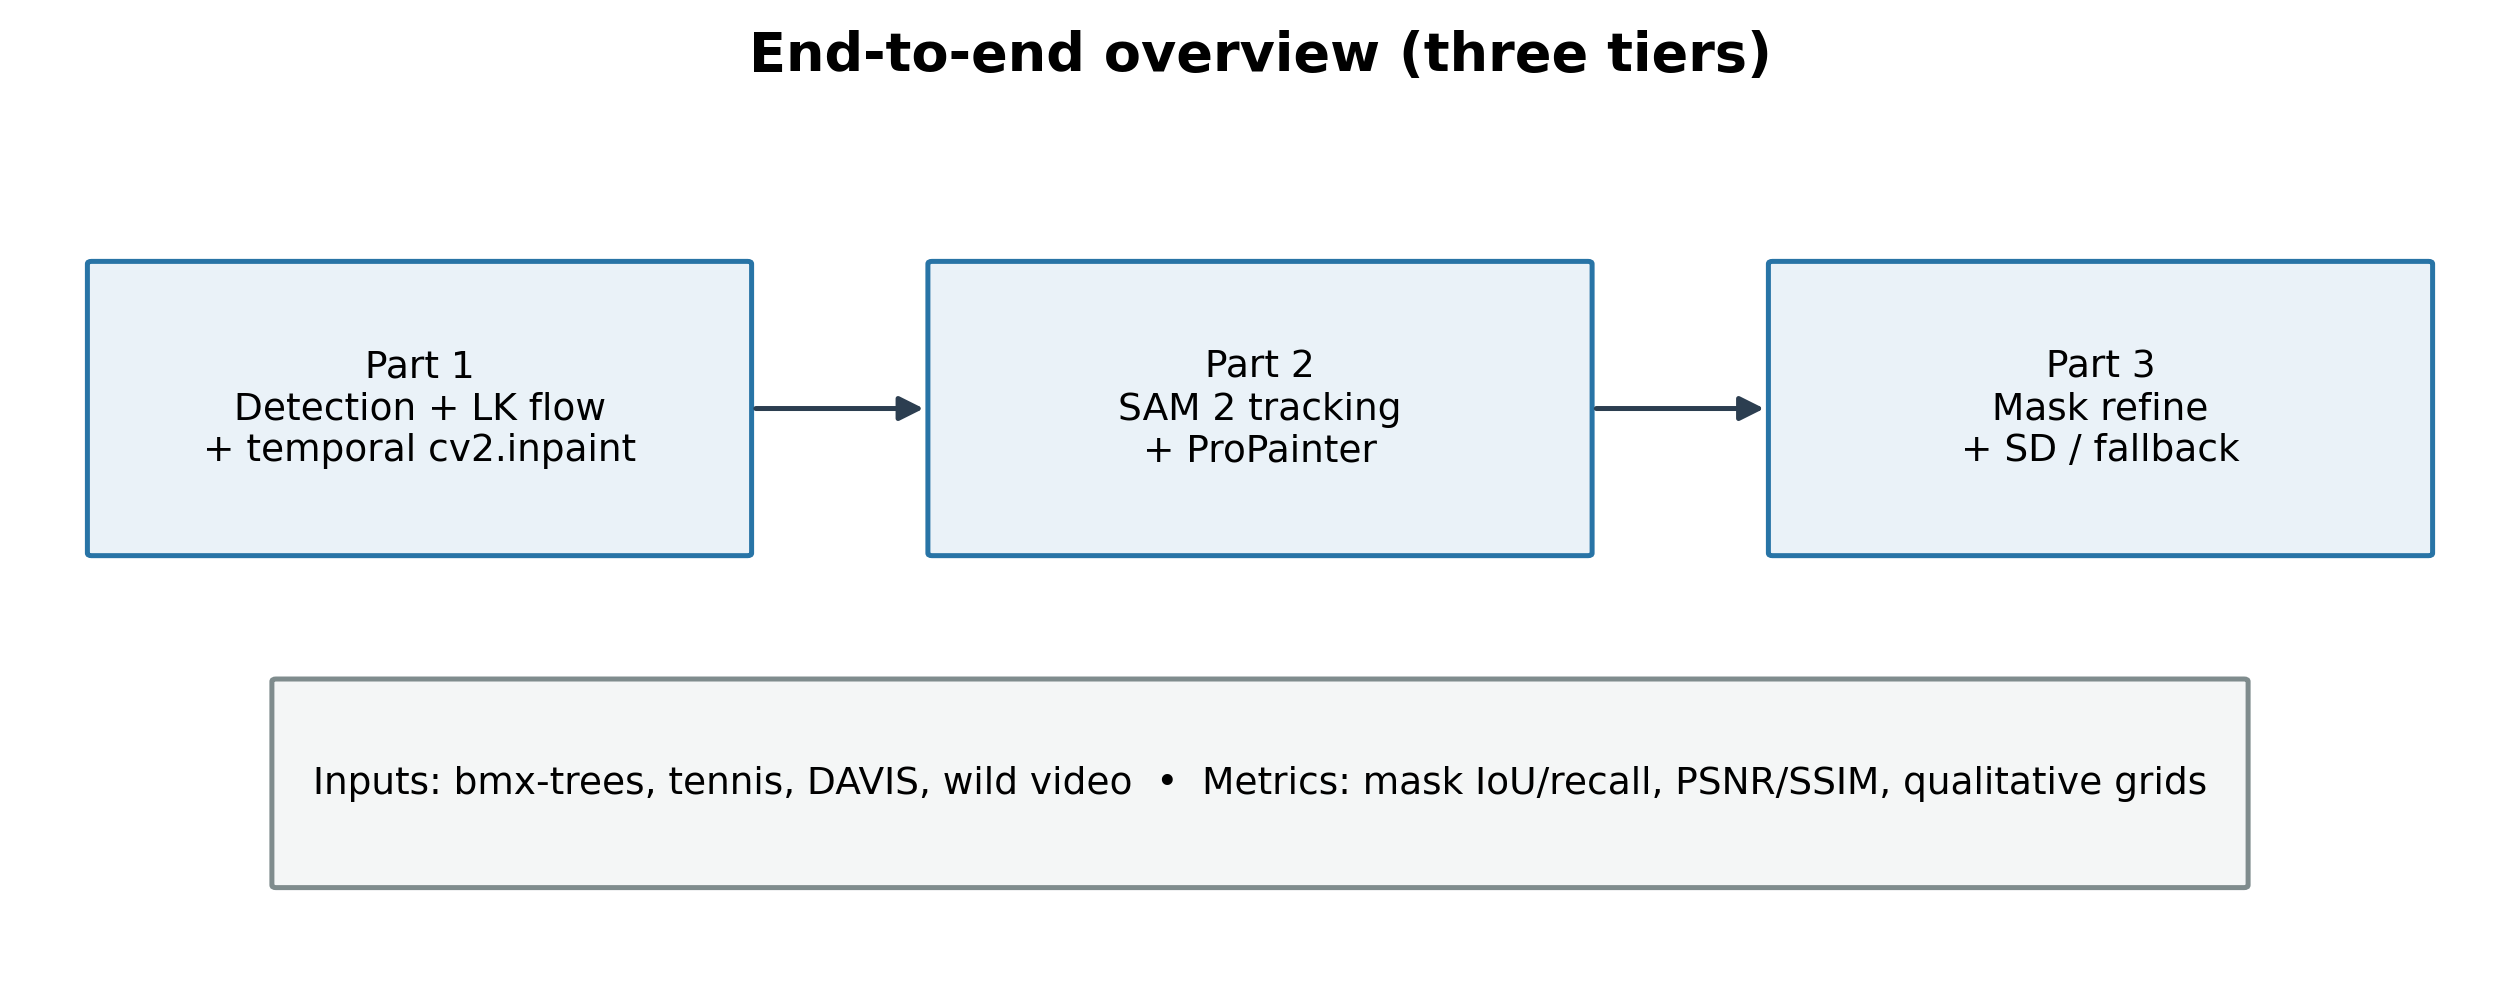
\includegraphics[width=\linewidth,height=0.28\textheight,keepaspectratio]{figures/pipeline_overview}
  \caption{Overall three-tier system. Part~1 uses classical CV, Part~2 uses SAM~2 and ProPainter, and Part~3 adds conservative mask refinement plus generative keyframe inpainting.}
  \label{fig:pipe_overview}
\end{figure}

\subsection{Part 1: Hand-crafted baseline}
\label{sec:part1}
Part~1 starts with YOLOv8-Seg masks for dynamic categories such as people, bicycles and vehicles. We then compute Lucas--Kanade sparse optical flow within each connected component. Components with insufficient reliable motion are treated as static and removed; to reduce failures under occlusion, the implementation keeps recent valid masks when tracked feature points disappear. Finally, masks are dilated to cover motion blur. The initial version used only \texttt{cv2.inpaint}, which produced mosaic-like blurred regions. We therefore added temporal background propagation: clean pixels are first borrowed from previous and future frames at the same or flow-warped locations when those pixels are unmasked; Telea/Navier--Stokes inpainting is used only as fallback.

\begin{figure}[H]
  \centering
  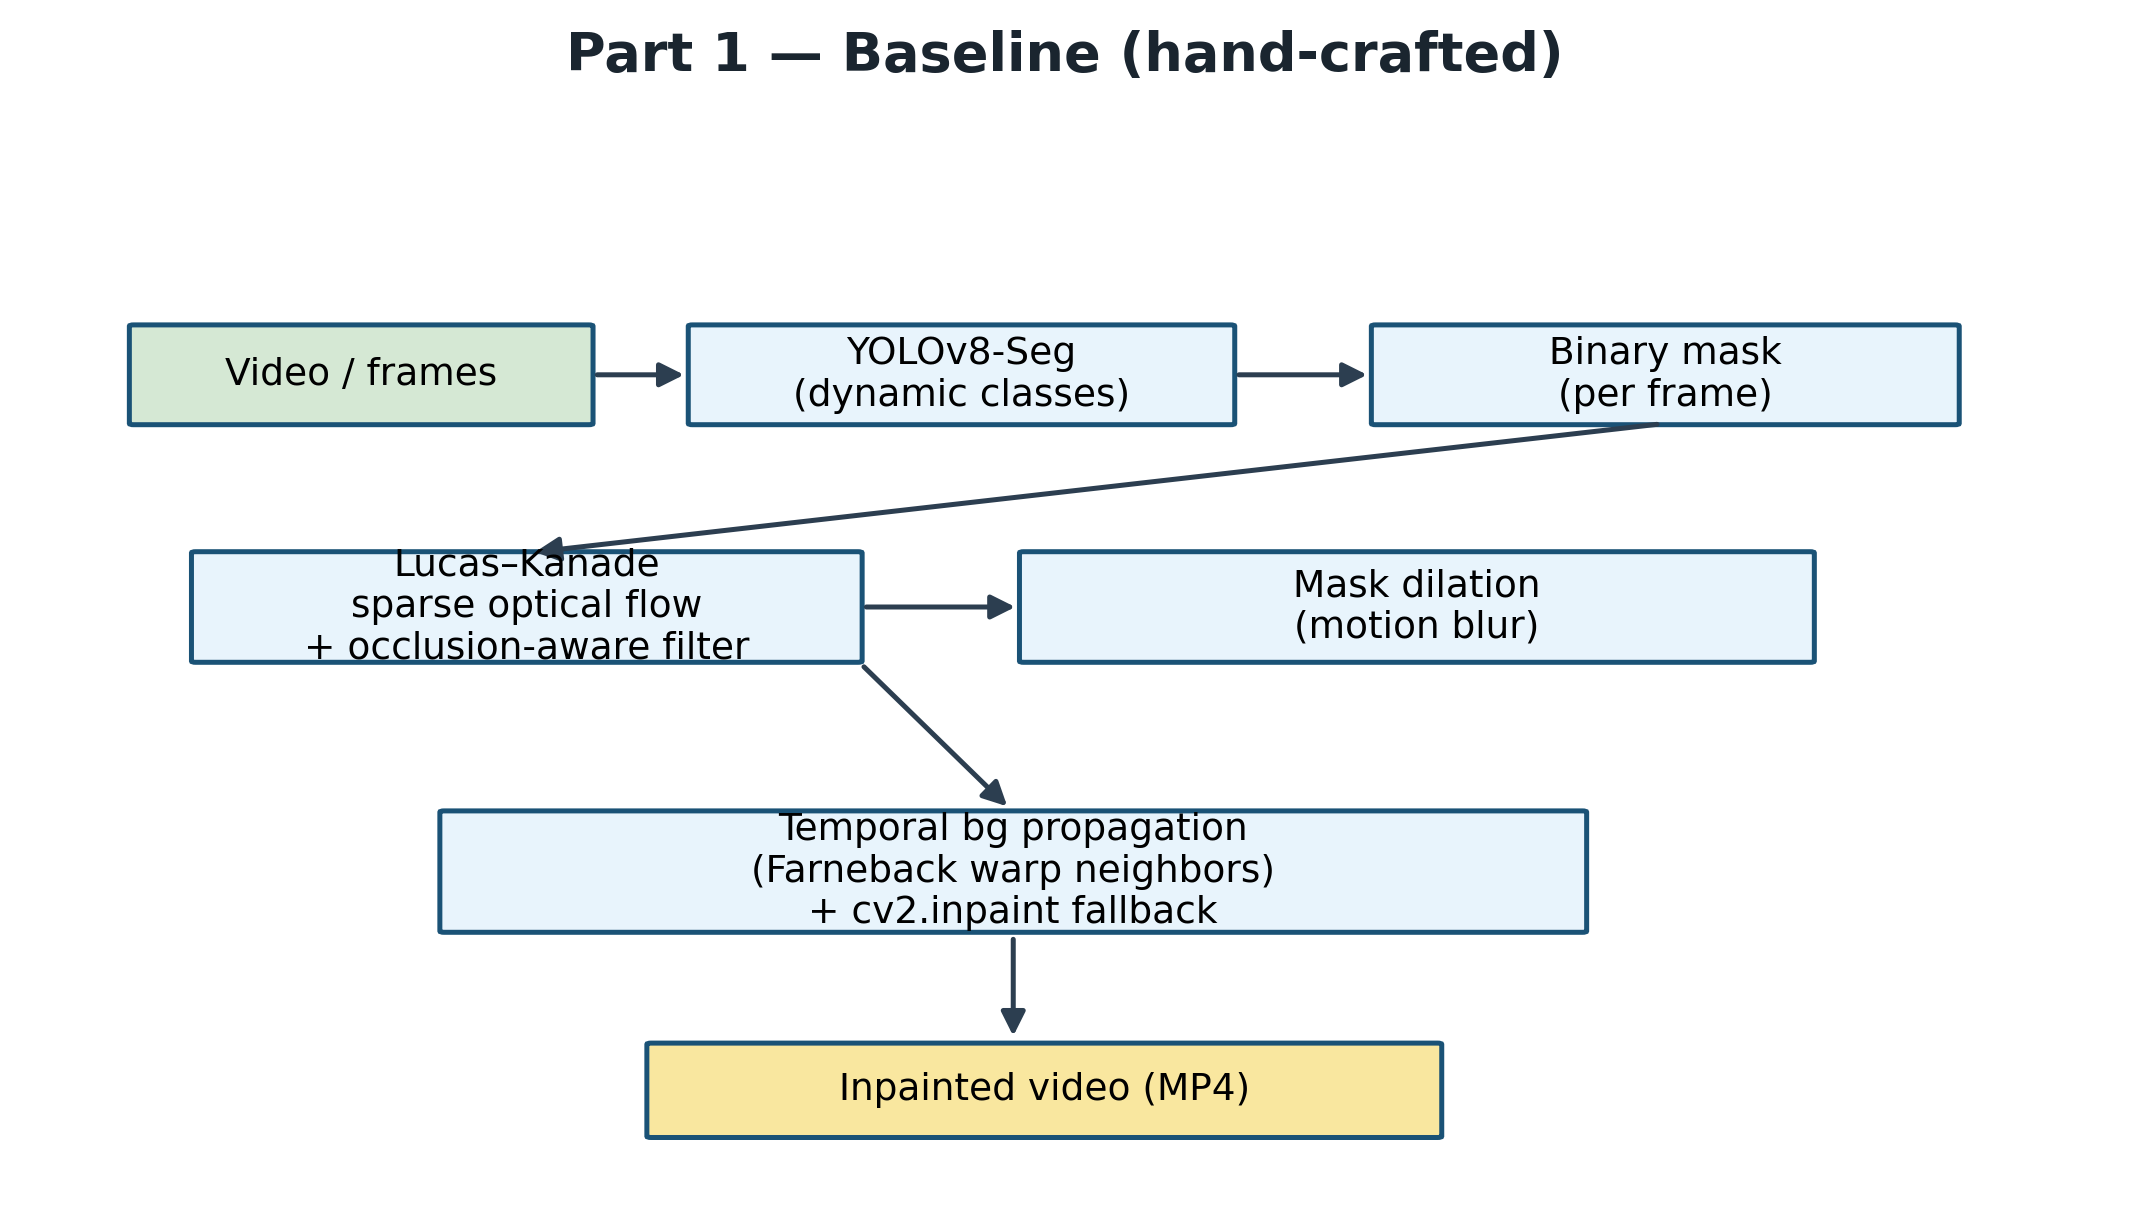
\includegraphics[width=\linewidth,height=0.27\textheight,keepaspectratio]{figures/pipeline_part1}
  \caption{Part~1 pipeline: YOLOv8-Seg, sparse optical-flow dynamic filtering, motion-blur dilation, temporal background propagation and OpenCV fallback inpainting.}
  \label{fig:part1}
\end{figure}

\subsection{Part 2: SAM~2 + ProPainter}
\label{sec:part2}
Part~2 targets the SOTA reproduction requirement. YOLOv8-Seg provides initial object proposals, and SAM~2 propagates them through video memory to obtain more coherent masks. During development we found that seeding only frame~0 fails when objects enter later, so the final implementation uses multi-frame initialization. The inpainting stage invokes ProPainter with FP16 inference to fit an RTX 4060 8GB GPU. A fallback flow-guided inpainter is also implemented; its propagation was corrected to avoid borrowing pixels from neighbor-frame masked regions.

\begin{figure}[H]
  \centering
  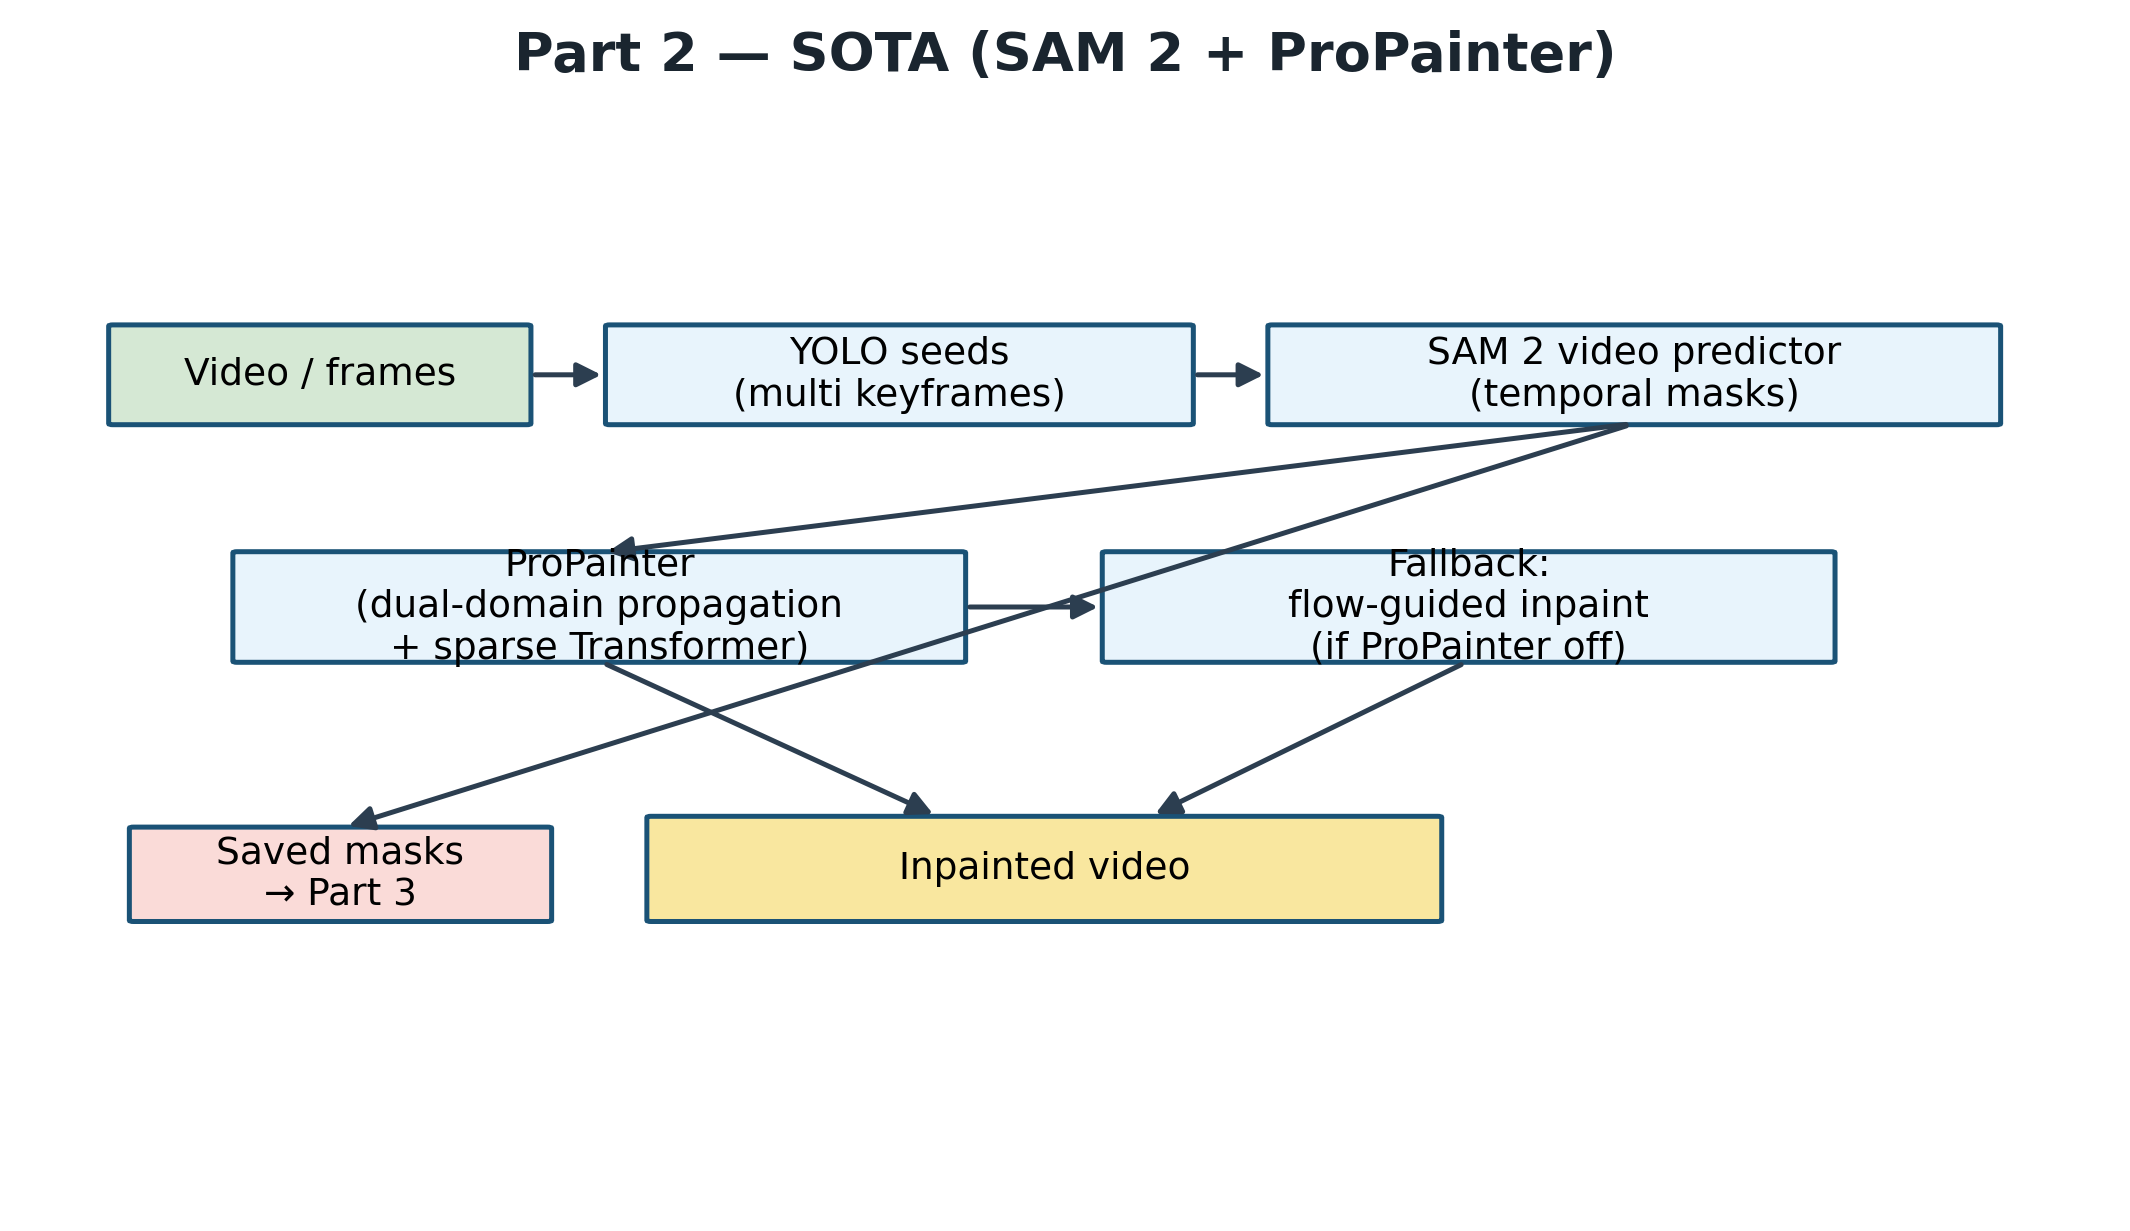
\includegraphics[width=\linewidth,height=0.27\textheight,keepaspectratio]{figures/pipeline_part2}
  \caption{Part~2 pipeline: SAM~2 video tracking and ProPainter dual-domain propagation with sparse temporal attention.}
  \label{fig:part2}
\end{figure}

\subsection{Part 3: Exploration and optimization}
\label{sec:part3}
Part~3 explores the optimization directions from the project handout. For mask upgrade, SAM~3 is discussed but not used directly because the required public package was unavailable; instead we implement a conservative fallback using light dilation, area-guarded GrabCut, and morphology. Aggressive open/close refinement lowered IoU in early trials, so the final version avoids changing SAM~2 boundaries unless the candidate mask stays within a small area ratio.

For generative inpainting, Stable Diffusion inpainting is applied only on selected keyframes. Non-keyframes are filled by optical-flow warping and interpolation between nearest generated keyframes. To reduce visible seams, the hard binary mask replacement was replaced with Gaussian feathering plus Poisson seamless cloning inside the confident region. This branch improves masked PSNR on nearly all evaluated sequences, but it can hallucinate inconsistent texture and still cannot guarantee true video-level temporal coherence.

\begin{figure}[H]
  \centering
  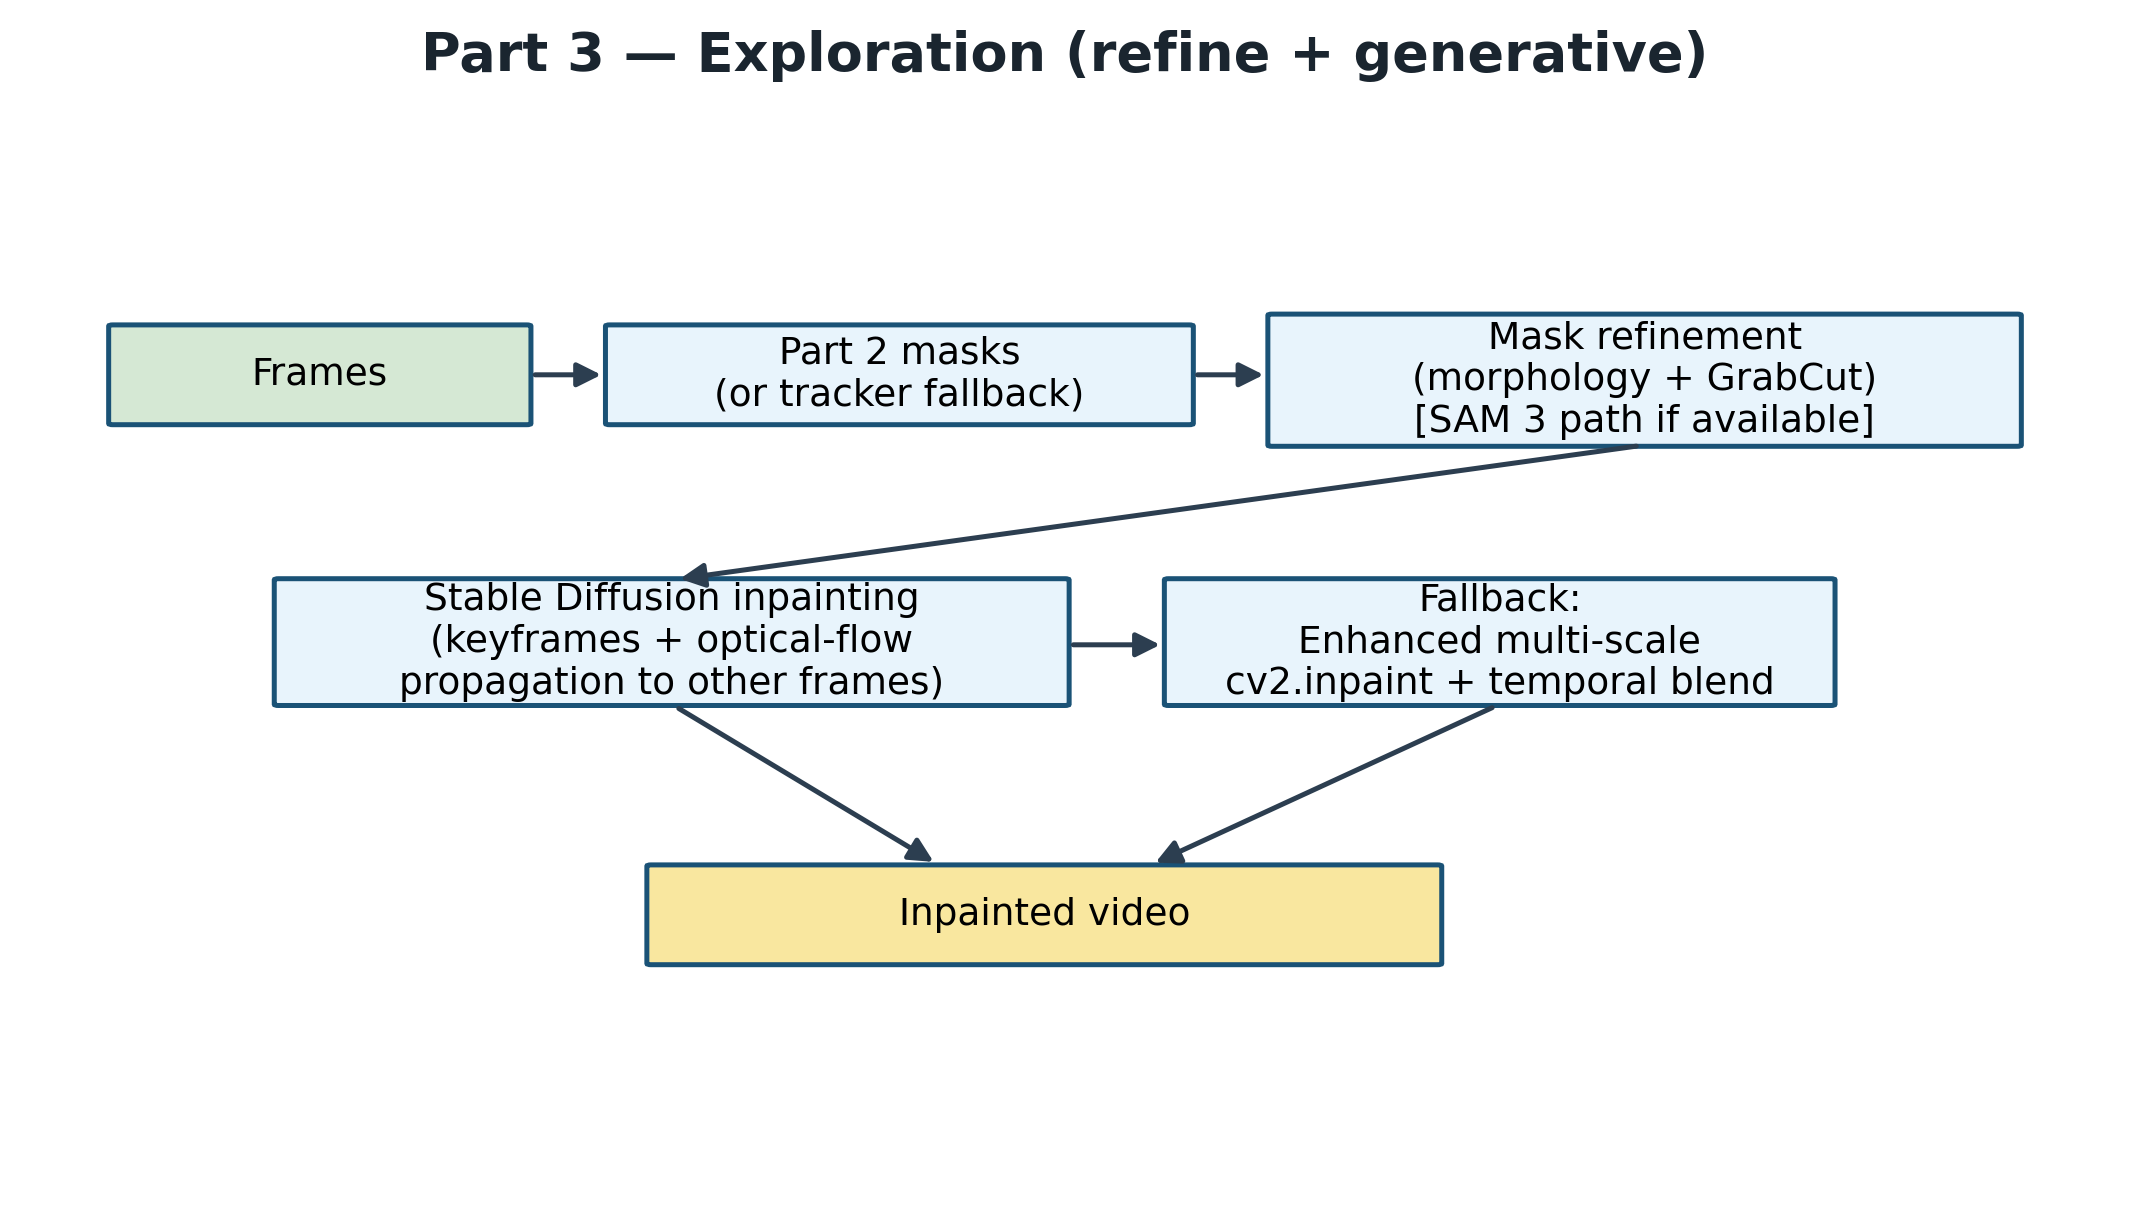
\includegraphics[width=\linewidth,height=0.27\textheight,keepaspectratio]{figures/pipeline_part3}
  \caption{Part~3 pipeline: conservative mask refinement, Stable Diffusion keyframes, optical-flow propagation, feathered alpha blending and Poisson seamless cloning.}
  \label{fig:part3}
\end{figure}

\subsection{Engineering details}
The implementation uses frame folders as the common representation instead of forcing every module to consume an encoded video. This avoids codec-dependent failures and makes it possible to inspect intermediate masks. All video readers and writers therefore handle both \texttt{.mp4} files and ordered image directories. For Windows paths containing non-ASCII characters, image I/O uses byte-buffer based OpenCV loading and saving rather than plain \texttt{cv2.imread}; otherwise DAVIS and wild-video paths under Chinese directory names can fail silently.

Mask storage is also standardized. Each part writes binary masks as numbered PNG files and writes \texttt{inpainted.mp4} under \texttt{results/partX/<sequence>/}. This directory convention is used by the evaluation script to load outputs automatically. For DAVIS annotations, masks are palette PNGs rather than ordinary binary masks, so the evaluator uses a dedicated DAVIS mask loader. This detail matters because treating palette indices as grayscale intensities changes IoU and recall.

The heavy models are isolated behind fallbacks. If SAM~2 is unavailable, Part~2 can fall back to YOLO masks with temporal smoothing; if ProPainter is unavailable, a flow-guided OpenCV inpainter is used; if diffusion fails to load, Part~3 falls back to multi-scale inpainting. These fallbacks are not intended to outperform the primary methods, but they keep the full project runnable on weaker machines and make failure cases explicit rather than hidden.

\subsection{Metric protocol and caveats}
For mask metrics, we compare predicted object masks with DAVIS or provided sample masks. We report mean IoU as $J_M$ and recall as $J_R$, following the terminology in the project handout. For restoration metrics, we report PSNR/SSIM against the available original frames. This is not a perfect measure of true background reconstruction because the original frames still contain the object; however, the same imperfect target is used for all three methods, so the metric remains useful for relative comparison. Masked-region PSNR/SSIM is more sensitive to the actual edited area, while full-frame PSNR/SSIM can be dominated by unchanged background pixels. We therefore include both, and rely on qualitative grids for final visual judgment.

\section{Experiments}
\label{sec:exp}
\subsection{Setup}
Experiments were run with Python 3.11 on Windows and an NVIDIA RTX 4060 8GB GPU. We evaluate the mandatory \texttt{bmx-trees}, \texttt{tennis}, and a self-captured wild clip. To exceed the minimum dataset scope, we additionally evaluate DAVIS-2017 sequences \texttt{crossing}, \texttt{car-shadow}, \texttt{blackswan}, \texttt{dance-jump}, and \texttt{bus}. The wild clip was resized to 480p frames to avoid OpenCV memory failures in dense temporal operations. For masks we report mean IoU and recall, corresponding to $J_M$ and $J_R$. For restoration we report PSNR and SSIM both on the full frame and on masked regions. Since these videos do not provide clean background ground truth, PSNR/SSIM compare the restored frame with the original occluded frame; the metric is useful for controlled comparison but must be interpreted with qualitative figures.

\subsection{Quantitative results}
Table~\ref{tab:mask} reports mask quality on sequences with available masks. Part~2 improves strongly over the hand-crafted baseline, especially on \texttt{dance-jump}. Part~3 sometimes reduces IoU because it intentionally dilates masks to cover motion blur and seams, but it improves recall or inpainting coverage on several sequences.

\begin{table}[t]
  \centering
  \scriptsize
  \caption{Mask quality (mean IoU / recall). Higher is better.}
  \label{tab:mask}
  \begin{tabular}{lccc}
    \toprule
    Sequence & Part~1 & Part~2 & Part~3 \\
    \midrule
    bmx-trees & .520 / .808 & \textbf{.629} / .899 & .530 / \textbf{.913} \\
    tennis & .435 / .436 & .417 / .417 & \textbf{.478} / \textbf{.478} \\
    car-shadow & .830 / .958 & \textbf{.940} / \textbf{.970} & .891 / .958 \\
    blackswan & .851 / .934 & .913 / .950 & \textbf{.927} / \textbf{.955} \\
    dance-jump & .377 / .825 & \textbf{.736} / \textbf{.928} & .711 / .924 \\
    bus & .787 / .951 & .853 / .920 & \textbf{.862} / .948 \\
    crossing & .718 / .934 & \textbf{.808} / \textbf{.946} & .719 / .903 \\
    \midrule
    Mean & .645 / .807 & \textbf{.757} / .861 & .731 / \textbf{.868} \\
    \bottomrule
  \end{tabular}
\end{table}

Table~\ref{tab:inpaint} reports masked-region PSNR/SSIM. Part~3 improves masked PSNR on every sequence because diffusion and seam-aware blending fill larger regions more smoothly. Part~2 remains visually strongest on many videos because ProPainter preserves temporal consistency better and avoids diffusion hallucination.

\begin{table}[t]
  \centering
  \scriptsize
  \caption{Masked-region inpainting quality: PSNR / SSIM. Higher is better.}
  \label{tab:inpaint}
  \begin{tabular}{lccc}
    \toprule
    Sequence & Part~1 & Part~2 & Part~3 \\
    \midrule
    bmx-trees & 10.83 / .206 & 10.92 / .473 & \textbf{12.75} / \textbf{.483} \\
    tennis & 9.42 / .529 & 8.49 / .566 & \textbf{11.80} / \textbf{.612} \\
    car-shadow & 9.97 / \textbf{.547} & 11.40 / .361 & \textbf{11.81} / .388 \\
    blackswan & 13.72 / .621 & 13.77 / .663 & \textbf{15.78} / \textbf{.695} \\
    dance-jump & 12.72 / .751 & 14.15 / \textbf{.751} & \textbf{14.20} / .649 \\
    bus & 9.24 / .442 & 9.54 / \textbf{.509} & \textbf{11.39} / .501 \\
    crossing & 11.34 / .745 & 10.21 / .756 & \textbf{12.55} / \textbf{.769} \\
    \midrule
    Mean & 11.03 / .549 & 11.21 / .583 & \textbf{12.90} / \textbf{.585} \\
    \bottomrule
  \end{tabular}
\end{table}

\subsection{Ablation and implementation lessons}
The development history exposed several practical lessons. The original Part~1 restored each frame independently with \texttt{cv2.inpaint}; visually, this behaved like a mosaic layer over the moving object. Adding temporal background propagation changed the failure mode: when a region was visible in nearby frames, the restored texture became sharper, while Telea inpainting remained only a fallback for never-visible holes. For masks, sparse optical flow was helpful for rejecting static detections, but naive point tracking failed under occlusion; keeping recent valid masks made the baseline more stable.

Part~2 benefited most from replacing per-frame detection with video memory. Seeding SAM~2 only at frame~0 was fragile, so we used detections from multiple frames. ProPainter also made clear why video inpainting differs from image inpainting: by propagating features and pixels through time, it can recover repeated background patterns that a spatial method cannot infer.

Part~3 was useful as an optimization study rather than a universal replacement for Part~2. Aggressive morphology and GrabCut degraded high-quality SAM~2 masks, so the final refiner is intentionally conservative: light dilation covers motion blur, and area checks reject unstable refinements. The most reliable improvement came from replacing hard mask pasting with feathered alpha blending and Poisson cloning. This mainly improves boundary appearance and masked PSNR, but does not remove all temporal drift.

\begin{table}[t]
  \centering
  \scriptsize
  \caption{Full-frame restoration quality: PSNR / SSIM. Higher is better.}
  \label{tab:full}
  \begin{tabular}{lccc}
    \toprule
    Sequence & Part~1 & Part~2 & Part~3 \\
    \midrule
    bmx-trees & 25.23 / .904 & 26.12 / .913 & \textbf{27.11} / \textbf{.923} \\
    tennis & 22.17 / .869 & 21.73 / .871 & \textbf{24.08} / \textbf{.885} \\
    car-shadow & 21.38 / .885 & 23.43 / .897 & \textbf{23.81} / \textbf{.904} \\
    blackswan & 23.19 / .864 & 23.44 / .868 & \textbf{25.21} / \textbf{.883} \\
    dance-jump & 20.33 / .816 & \textbf{24.54} / .899 & 24.42 / \textbf{.900} \\
    bus & 15.85 / .763 & 16.98 / \textbf{.802} & \textbf{18.55} / \textbf{.802} \\
    crossing & 21.70 / .888 & 21.03 / .888 & \textbf{23.20} / \textbf{.905} \\
    \midrule
    Mean & 21.41 / .855 & 22.47 / .877 & \textbf{23.77} / \textbf{.886} \\
    \bottomrule
  \end{tabular}
\end{table}

\subsection{Qualitative comparison}
Figures~\ref{fig:qual_bmx}--\ref{fig:qual_carshadow} show representative comparison grids near the corresponding analysis. On \texttt{bmx-trees}, Part~1 removes objects but leaves blurry texture and ghosting. Part~2 better preserves background structure through temporal propagation. Part~3 often gives smoother filled regions and less visible mask boundary, but may synthesize texture that does not perfectly match neighboring frames. On the wild clip, the three-part comparison confirms generalization beyond packaged data, although no ground-truth mask exists for masked IoU.

The qualitative results also explain some metric disagreements. On \texttt{car-shadow}, Part~2 produces an accurate car mask, but the cast shadow remains because neither SAM~2 nor DAVIS annotations include shadows as part of the object. Part~3's light dilation covers slightly more boundary pixels and improves masked PSNR, but it still cannot remove a shadow that is outside the mask. On \texttt{crossing}, Part~2 has better mask IoU, yet Part~3 obtains higher inpainting PSNR because the generative branch fills the pedestrian region with smoother road texture. This supports using both mask metrics and restoration metrics: a good mask is necessary, but the inpainting model still determines whether the missing background looks natural.

For the wild video, we treat the results primarily as a generalization test. The clip contains stronger camera-specific noise and resolution constraints than the packaged samples. The original 720p video caused memory pressure in dense optical-flow and diffusion stages, so it was resized to 480p before processing. The comparison grid shows that the pipeline still detects and removes the main moving objects, but artifacts become more visible in areas with shadows and non-rigid motion. This is the main real-world failure mode we would target next.

\begin{figure}[H]
  \centering
  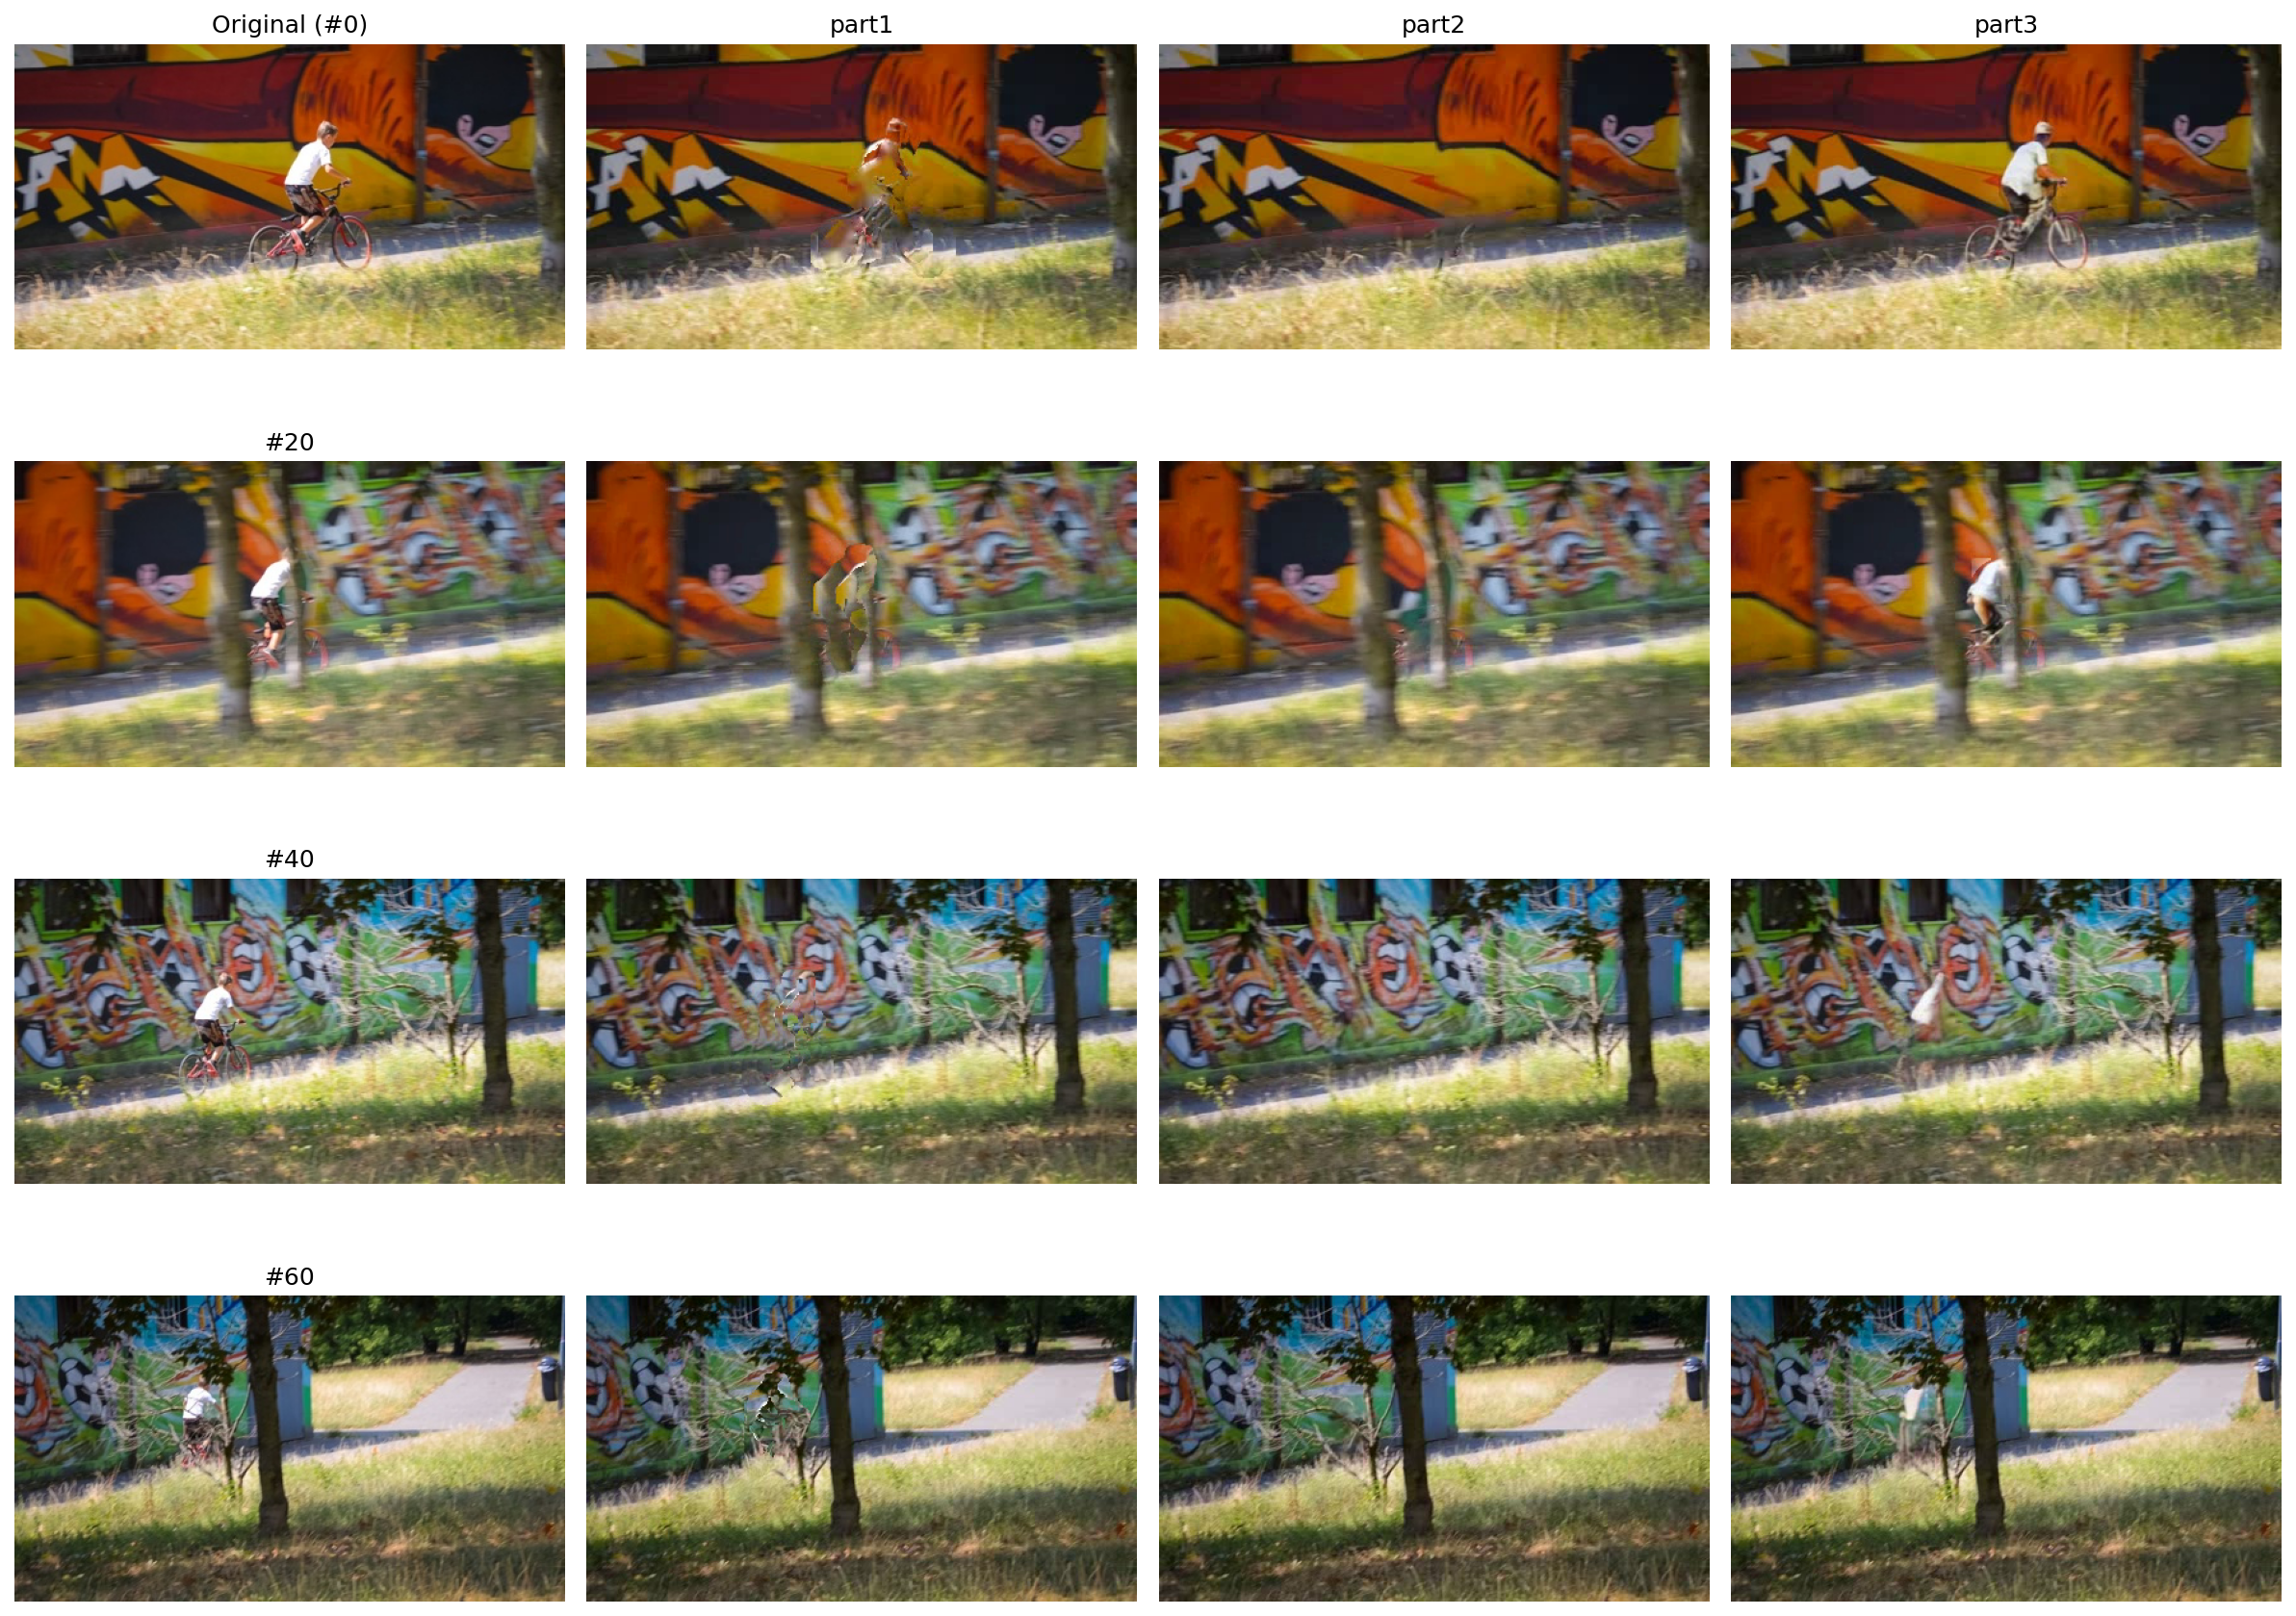
\includegraphics[width=\linewidth,height=0.16\textheight,keepaspectratio]{figures/comparison_bmx-trees}
  \caption{Mandatory sample result on \texttt{bmx-trees}.}
  \label{fig:qual_bmx}
\end{figure}

\begin{figure}[H]
  \centering
  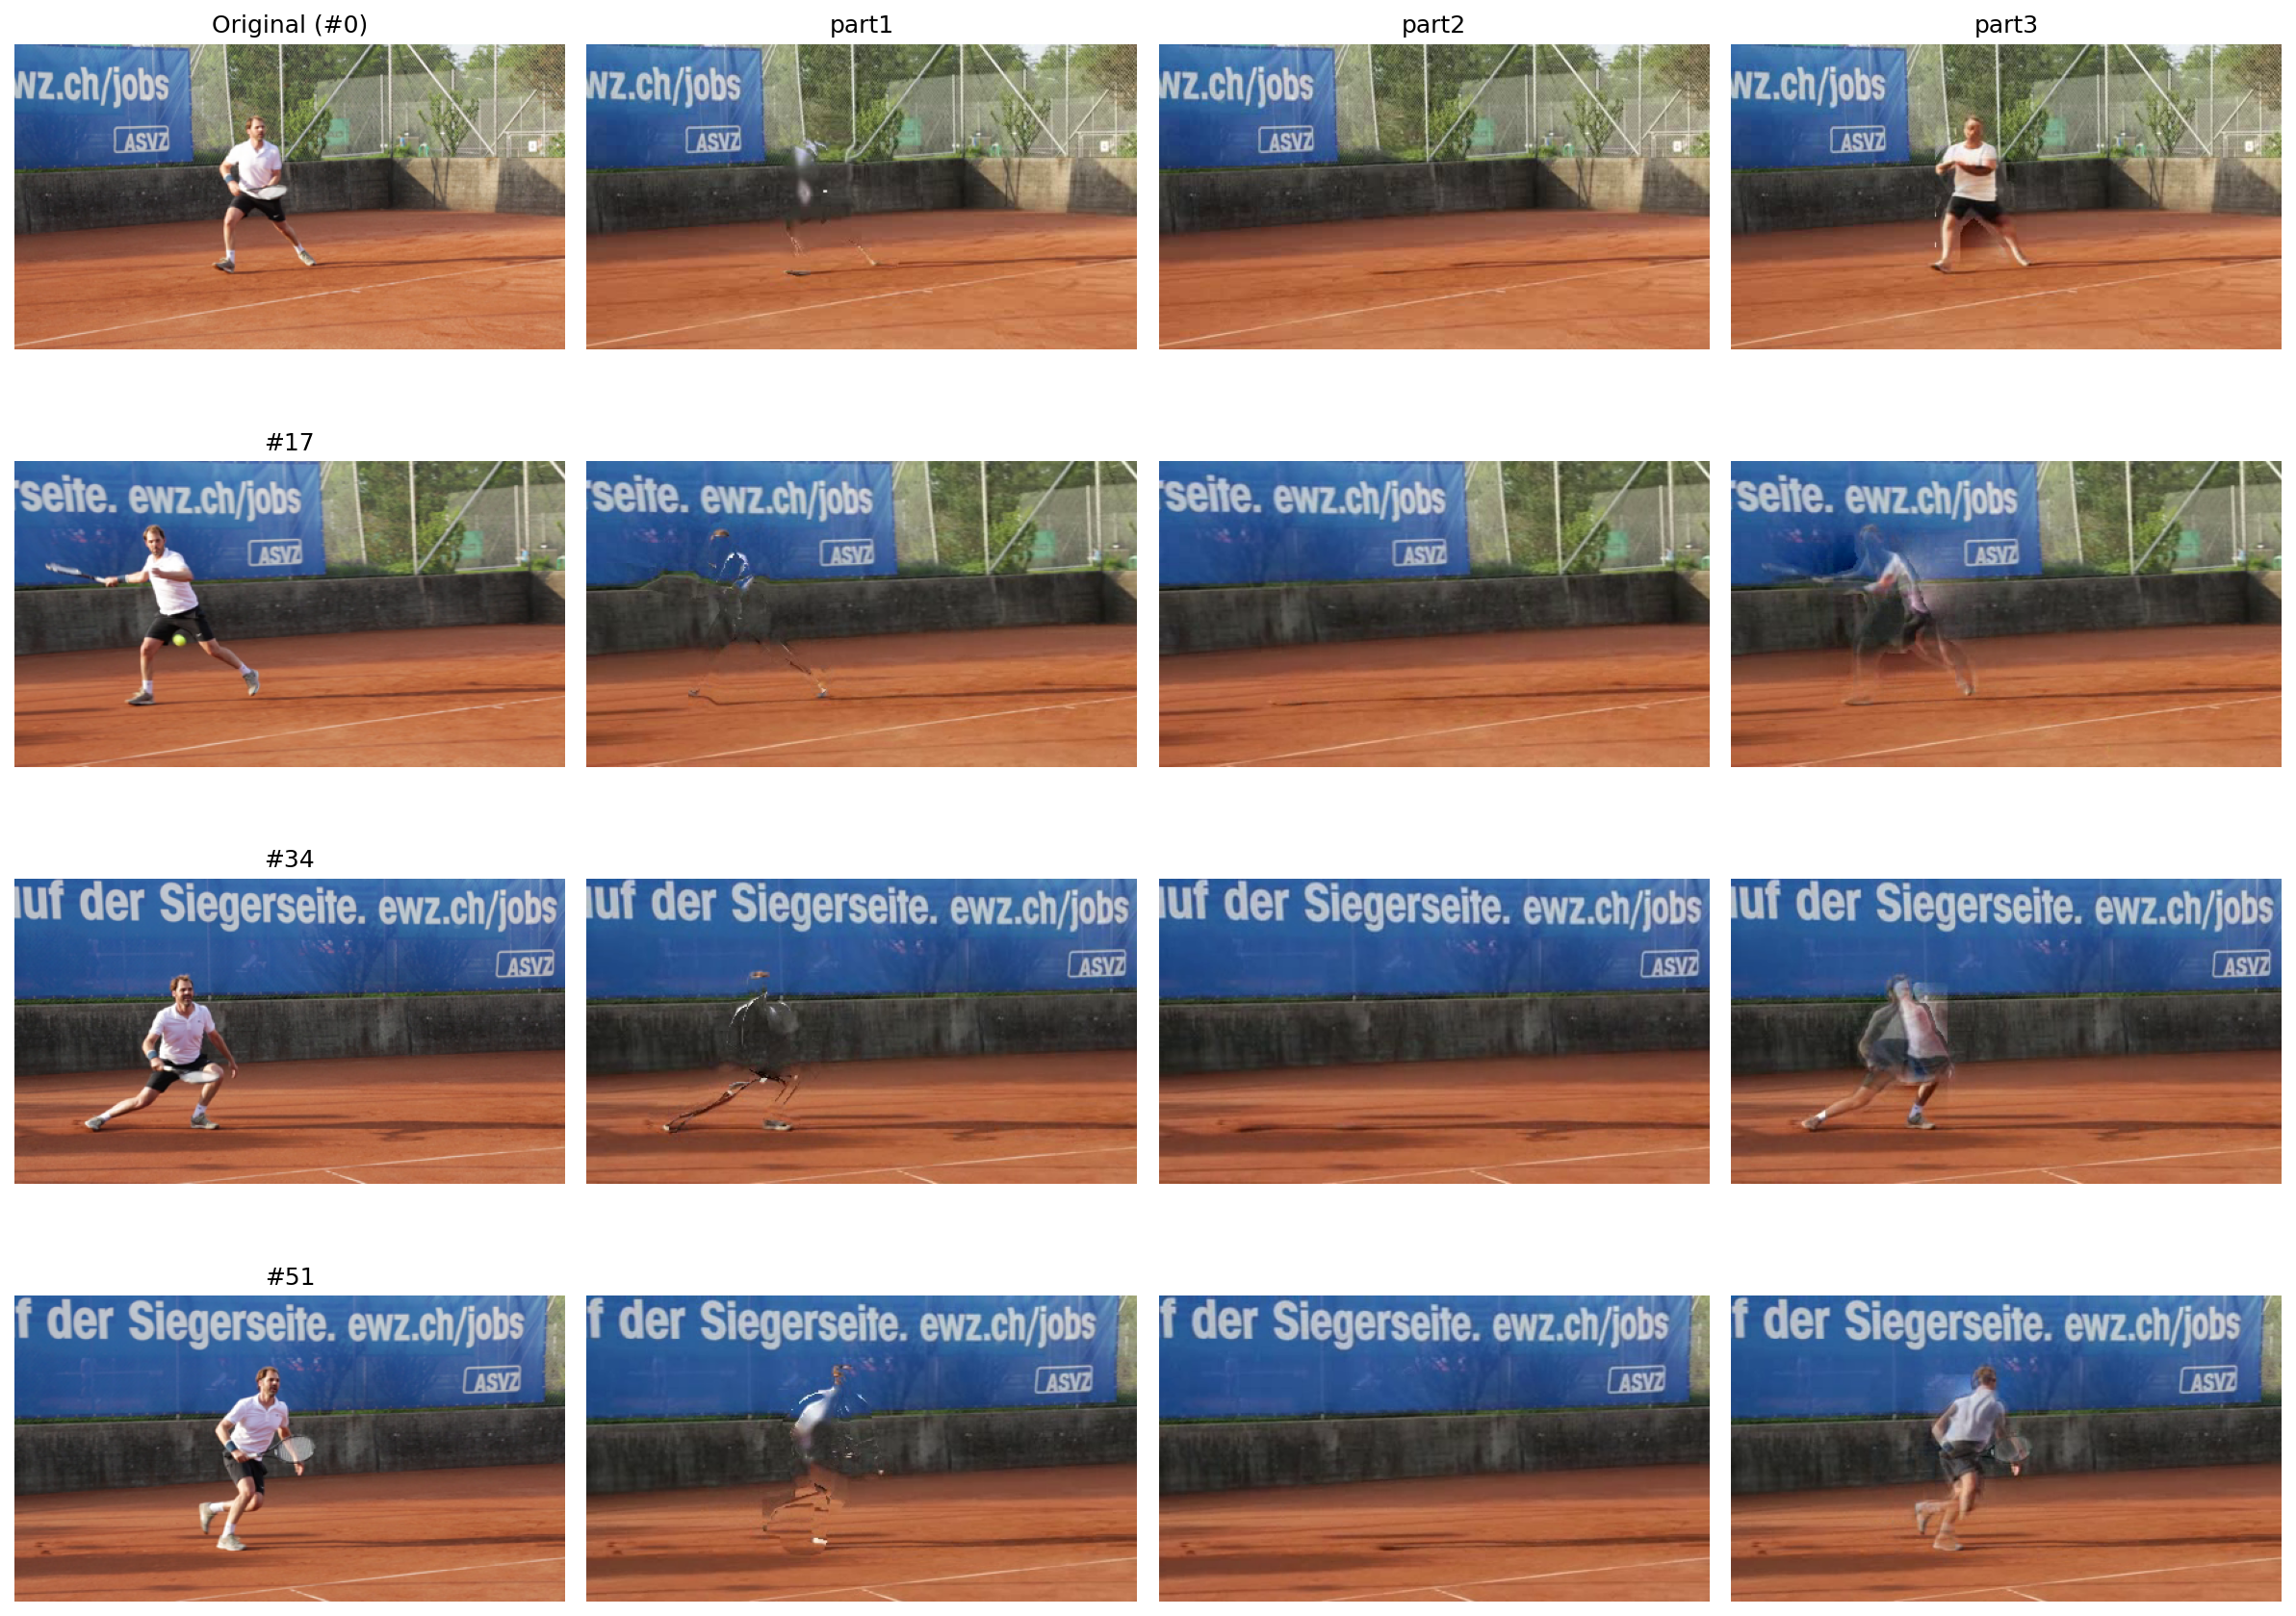
\includegraphics[width=\linewidth,height=0.16\textheight,keepaspectratio]{figures/comparison_tennis}
  \caption{Mandatory sample result on \texttt{tennis}.}
  \label{fig:qual_tennis}
\end{figure}

\begin{figure}[H]
  \centering
  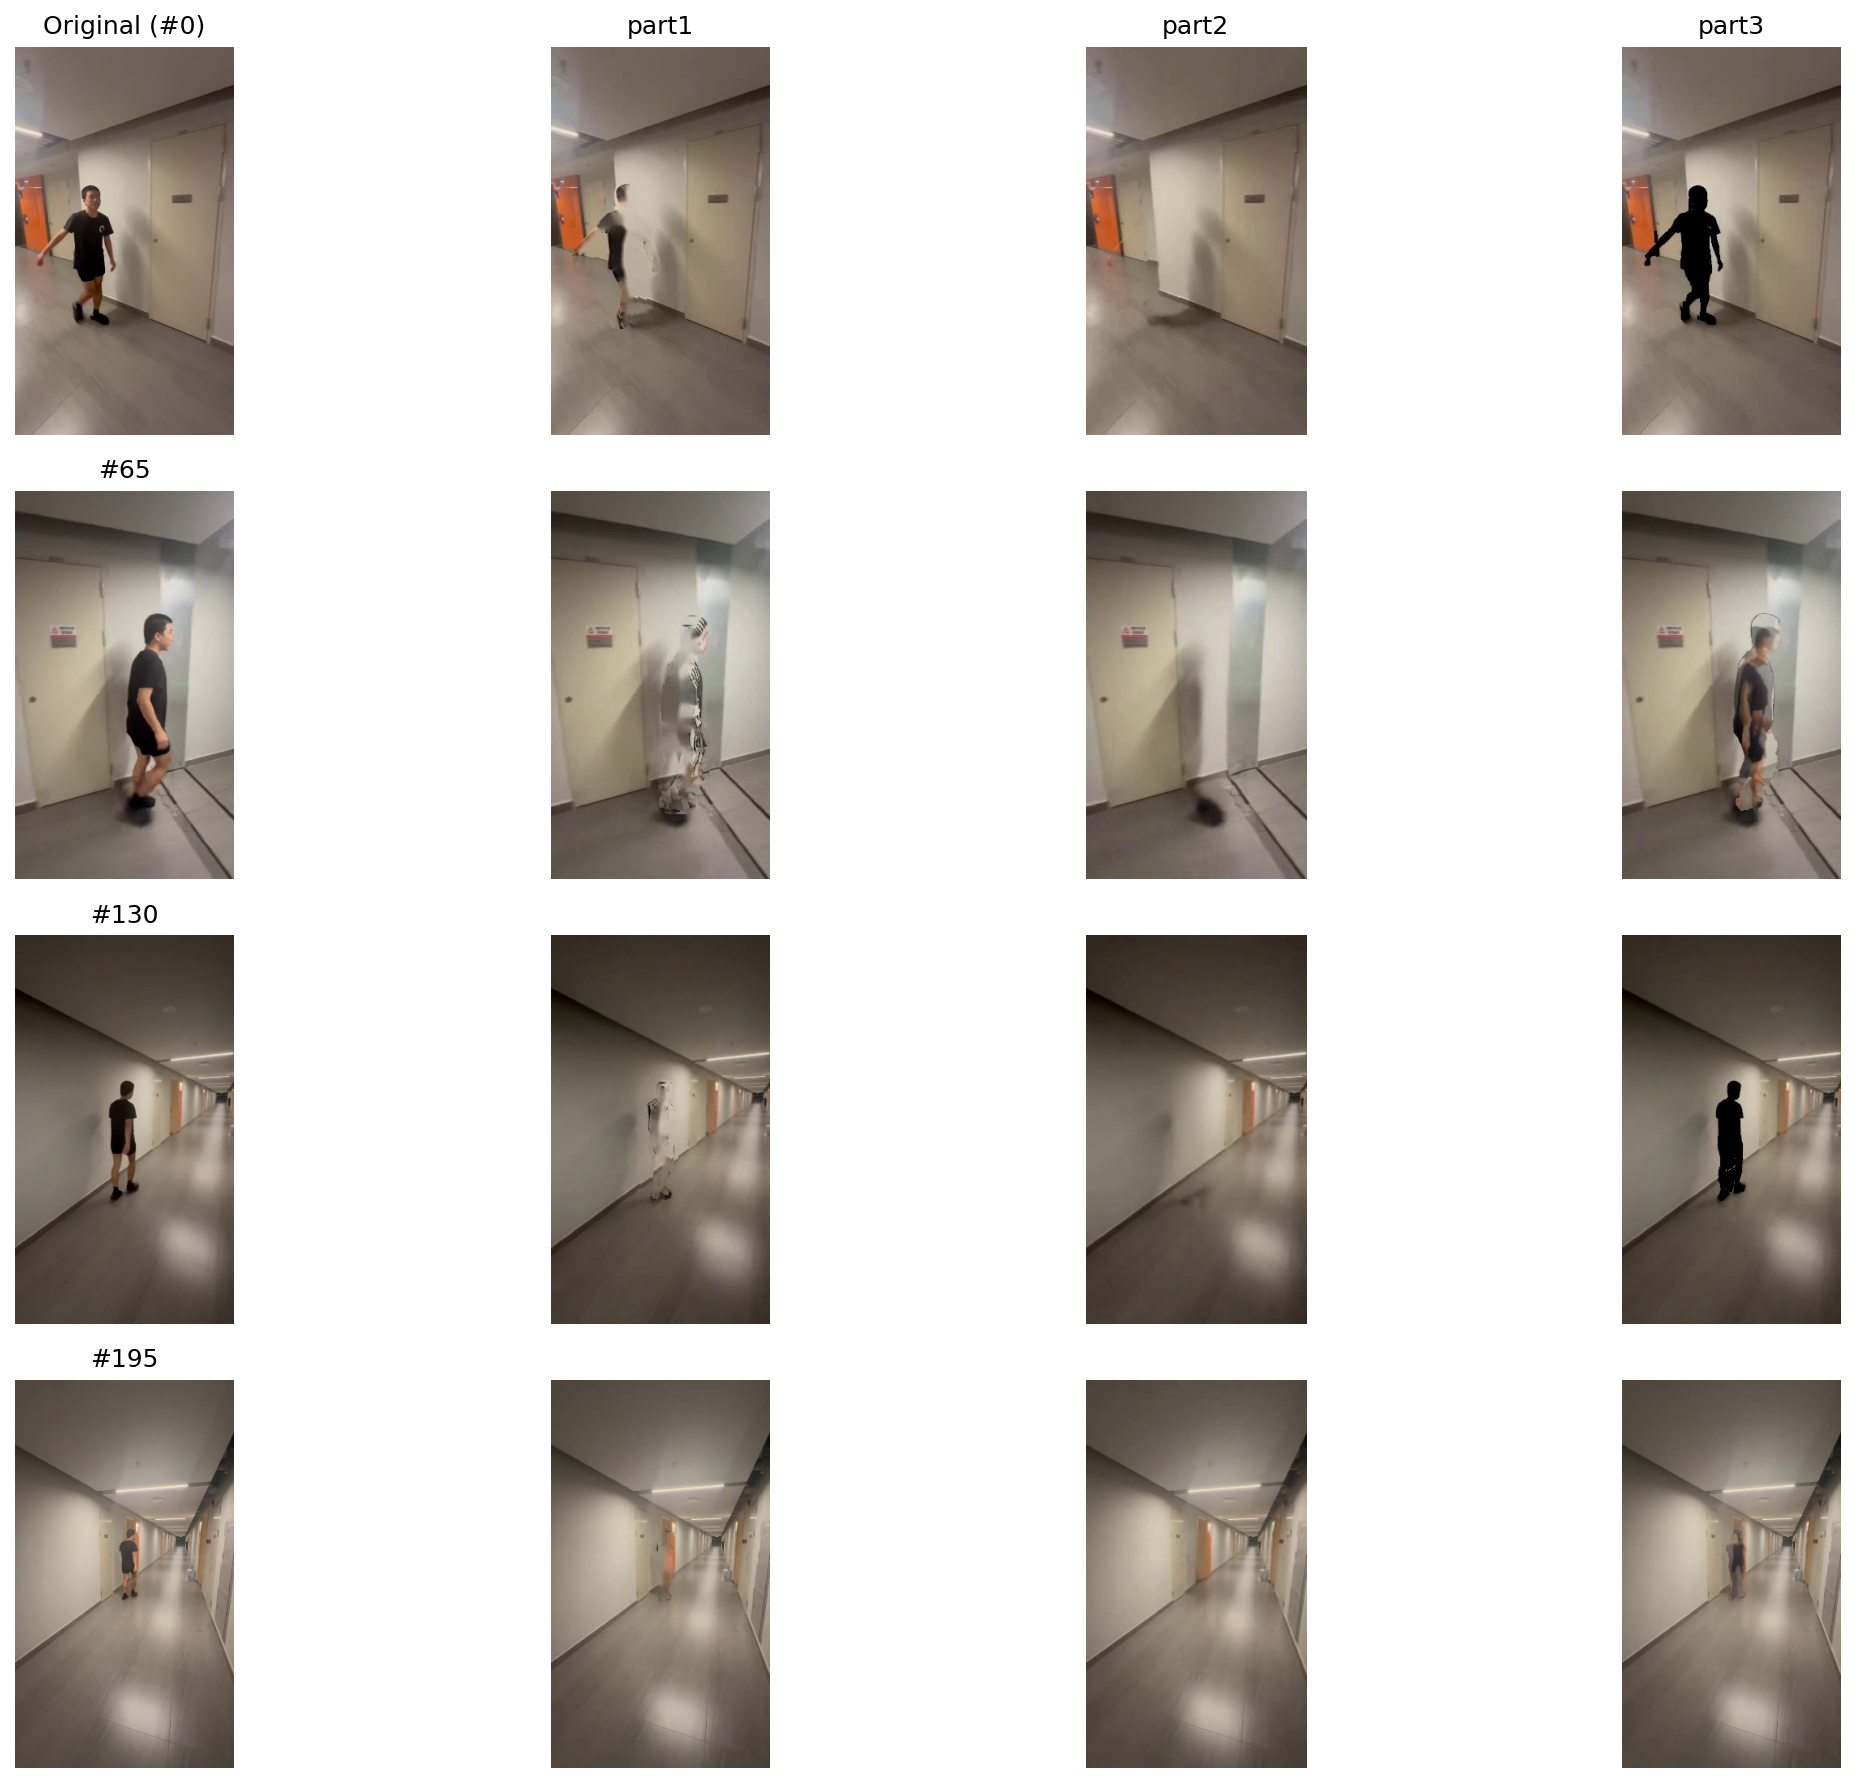
\includegraphics[width=\linewidth,height=0.16\textheight,keepaspectratio]{figures/comparison_wild_video}
  \caption{Self-captured wild-video result.}
  \label{fig:qual_wild}
\end{figure}

\begin{figure}[H]
  \centering
  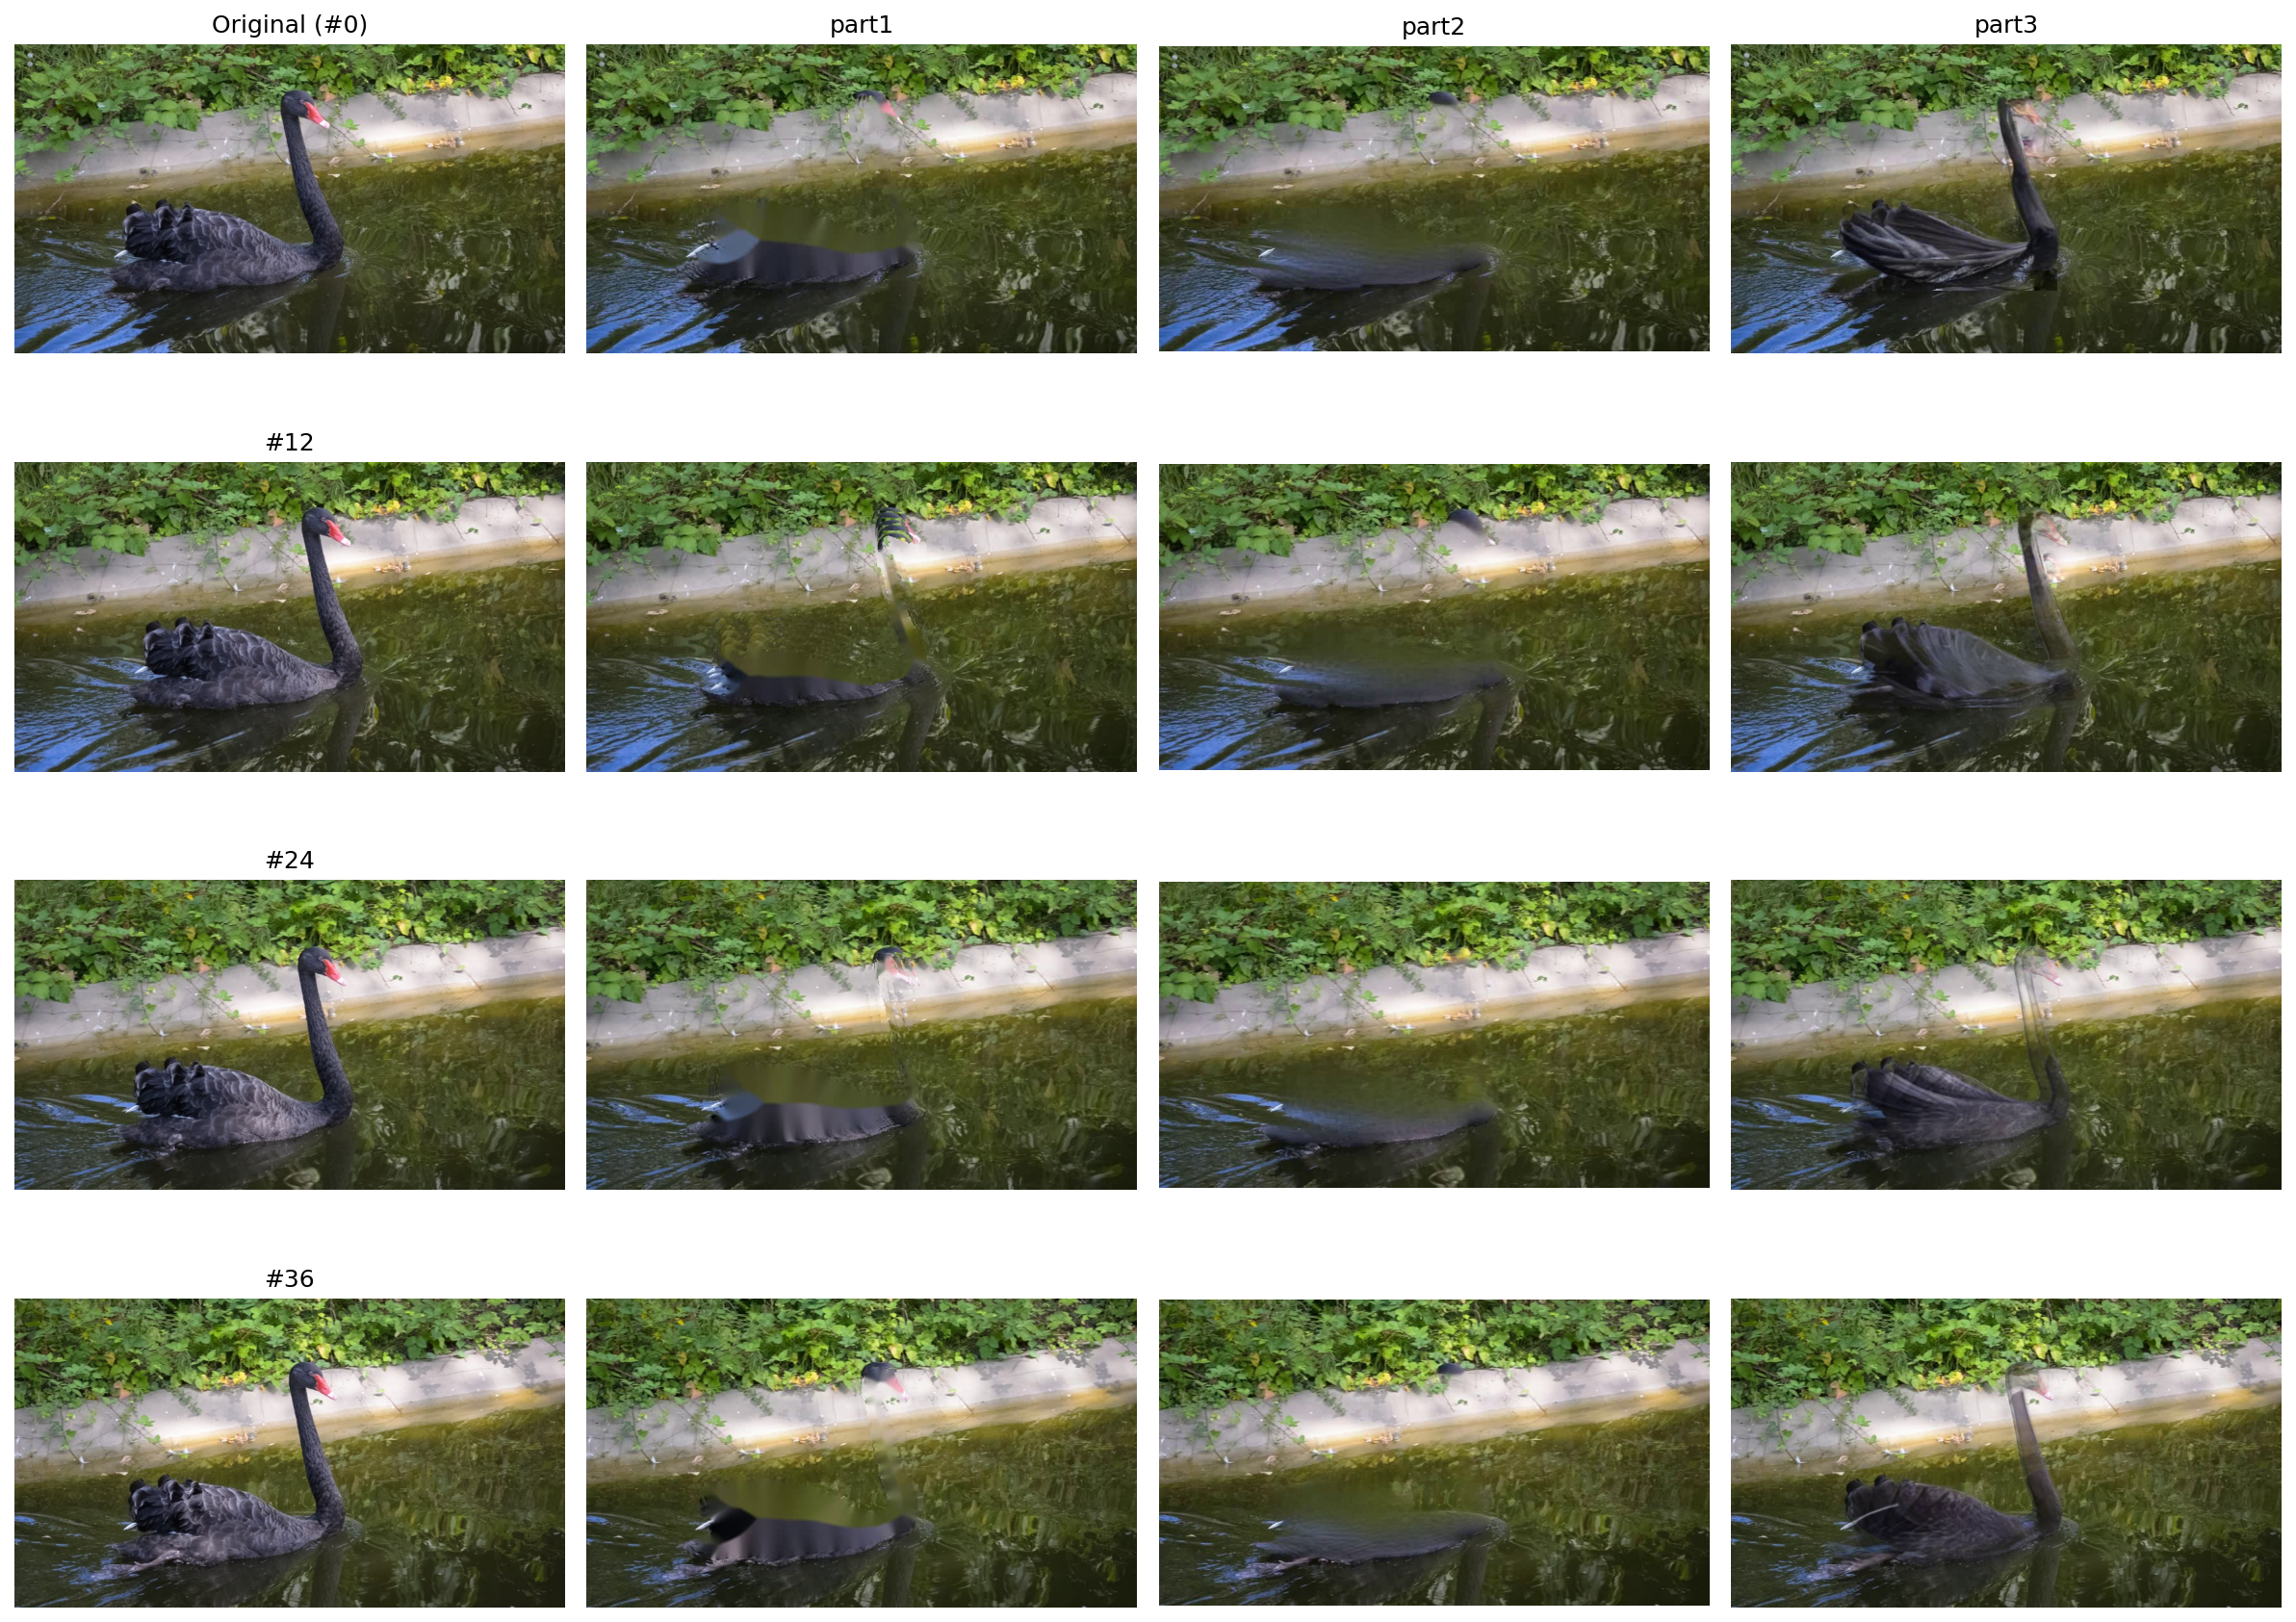
\includegraphics[width=\linewidth,height=0.16\textheight,keepaspectratio]{figures/comparison_blackswan}
  \caption{Additional DAVIS result on \texttt{blackswan}.}
  \label{fig:qual_blackswan}
\end{figure}

\begin{figure}[H]
  \centering
  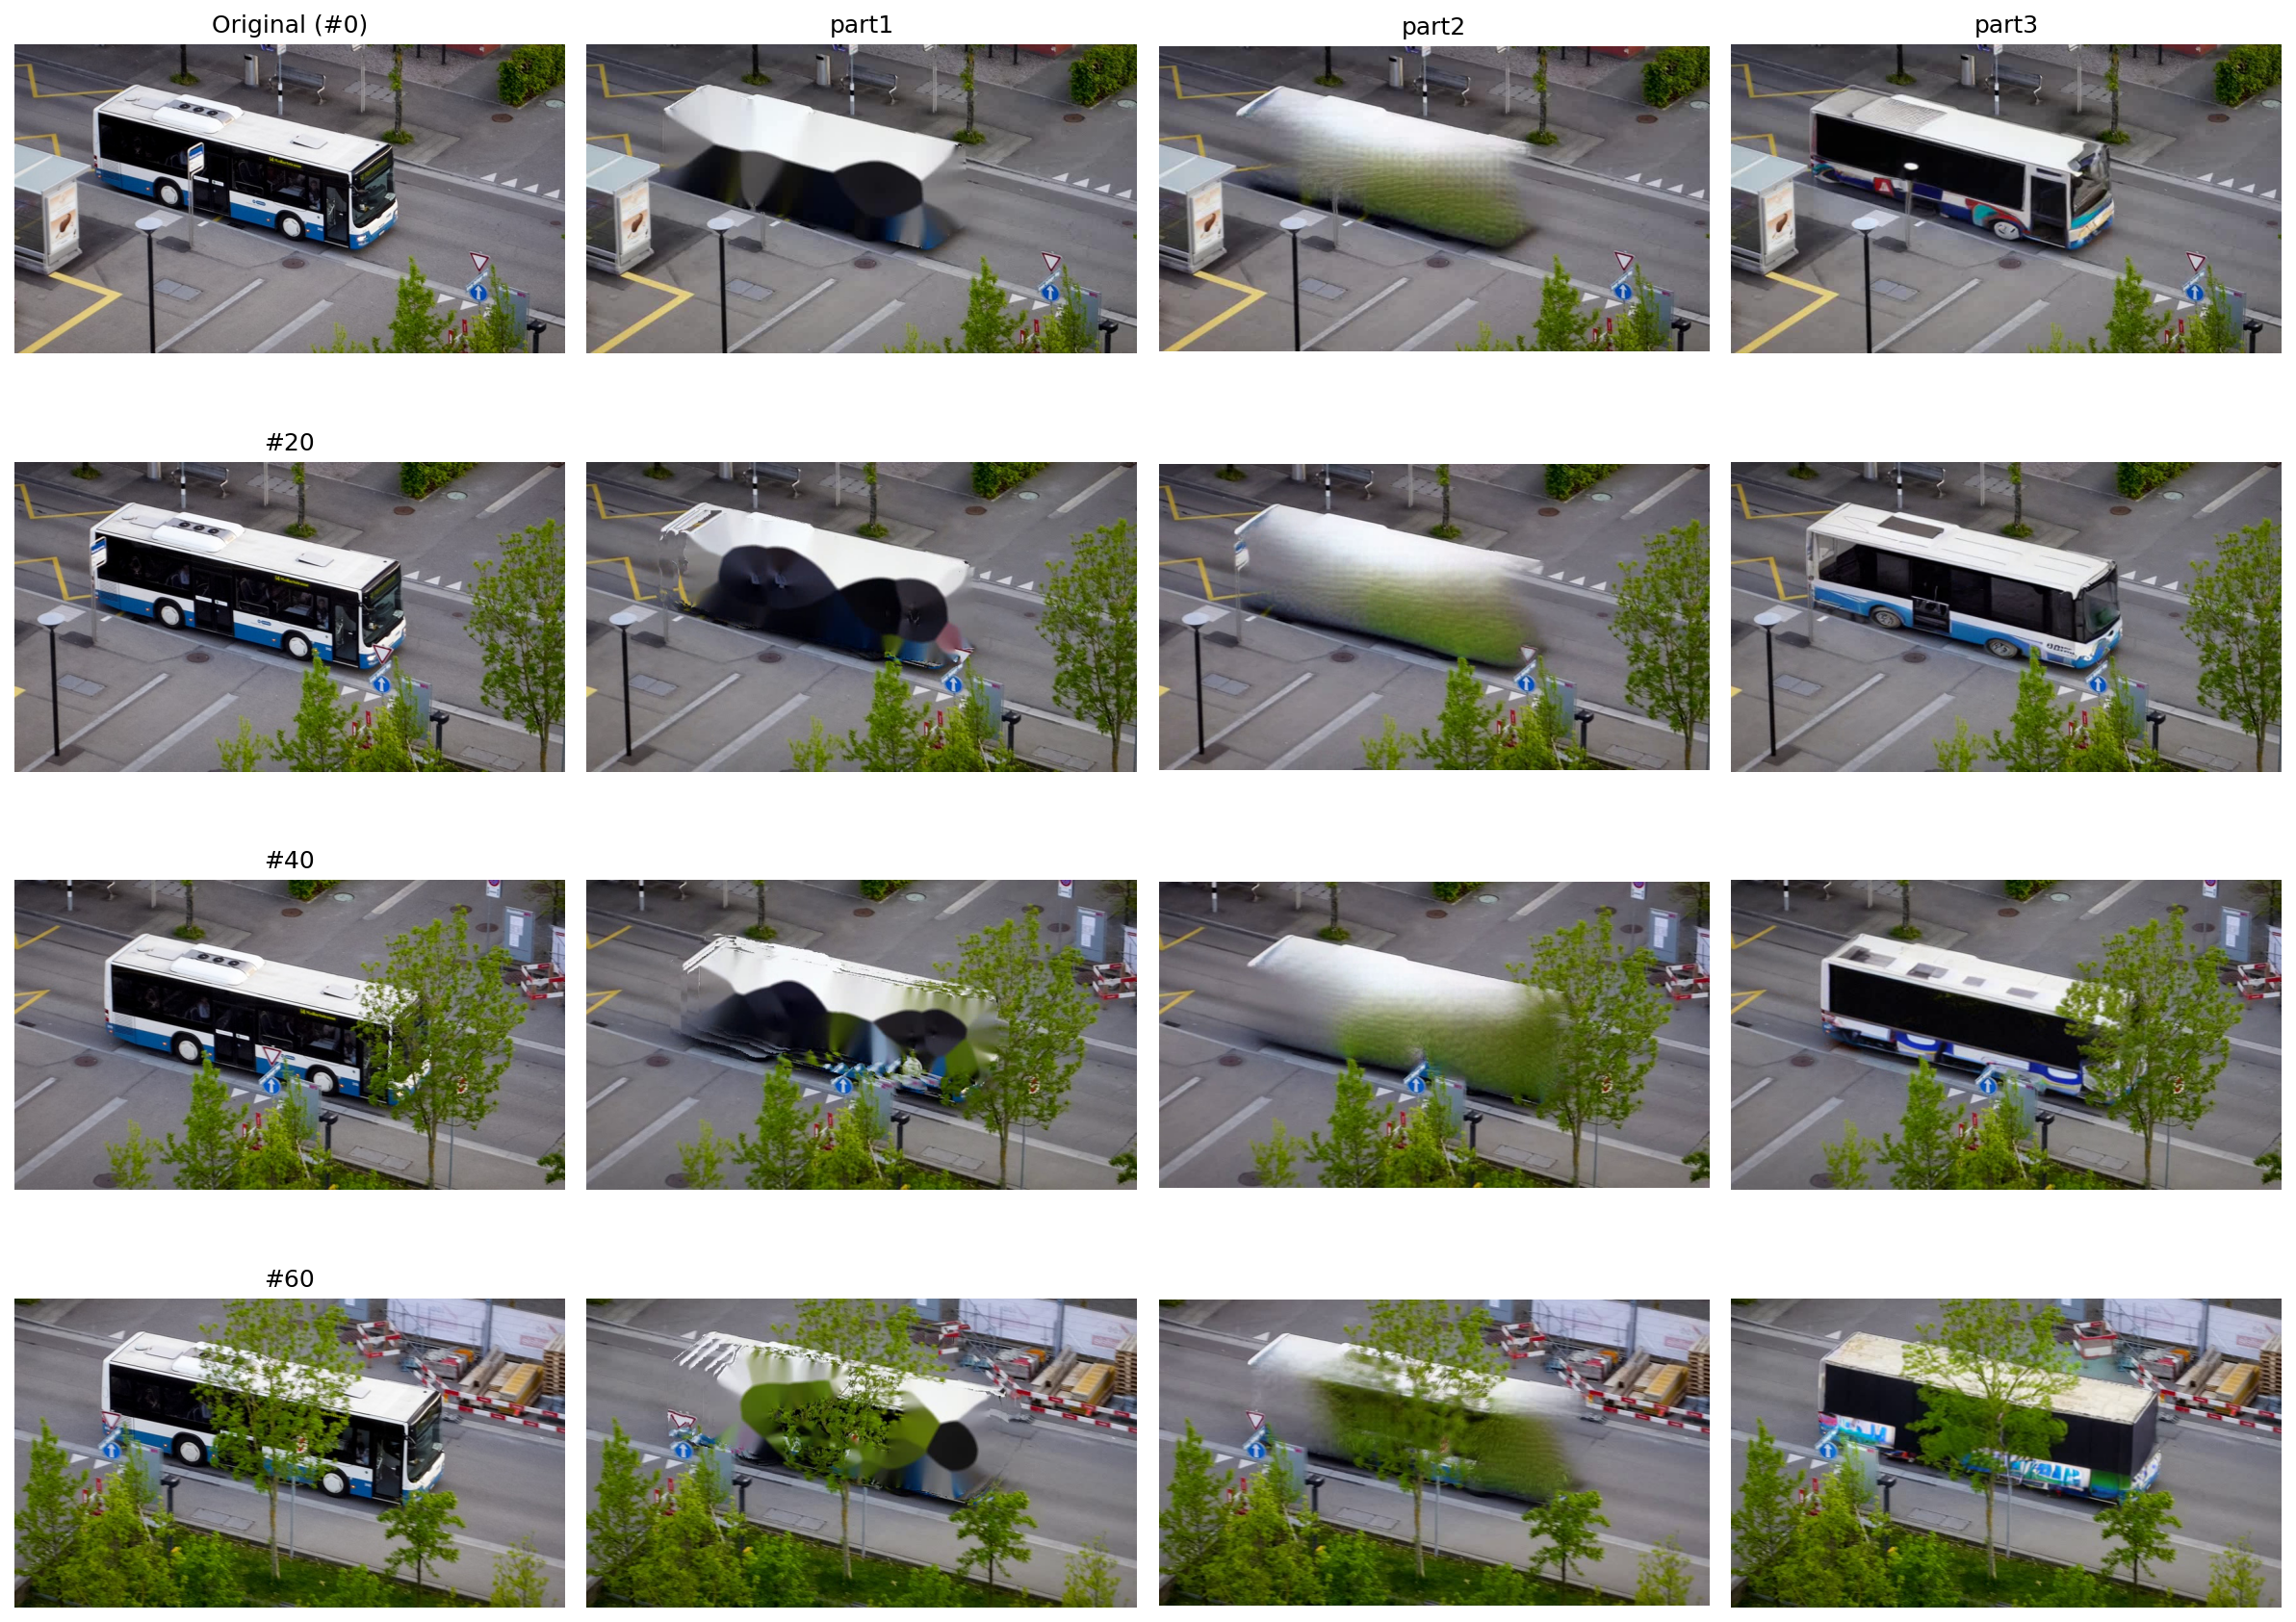
\includegraphics[width=\linewidth,height=0.16\textheight,keepaspectratio]{figures/comparison_bus}
  \caption{Additional DAVIS result on \texttt{bus}.}
  \label{fig:qual_bus}
\end{figure}

\begin{figure}[H]
  \centering
  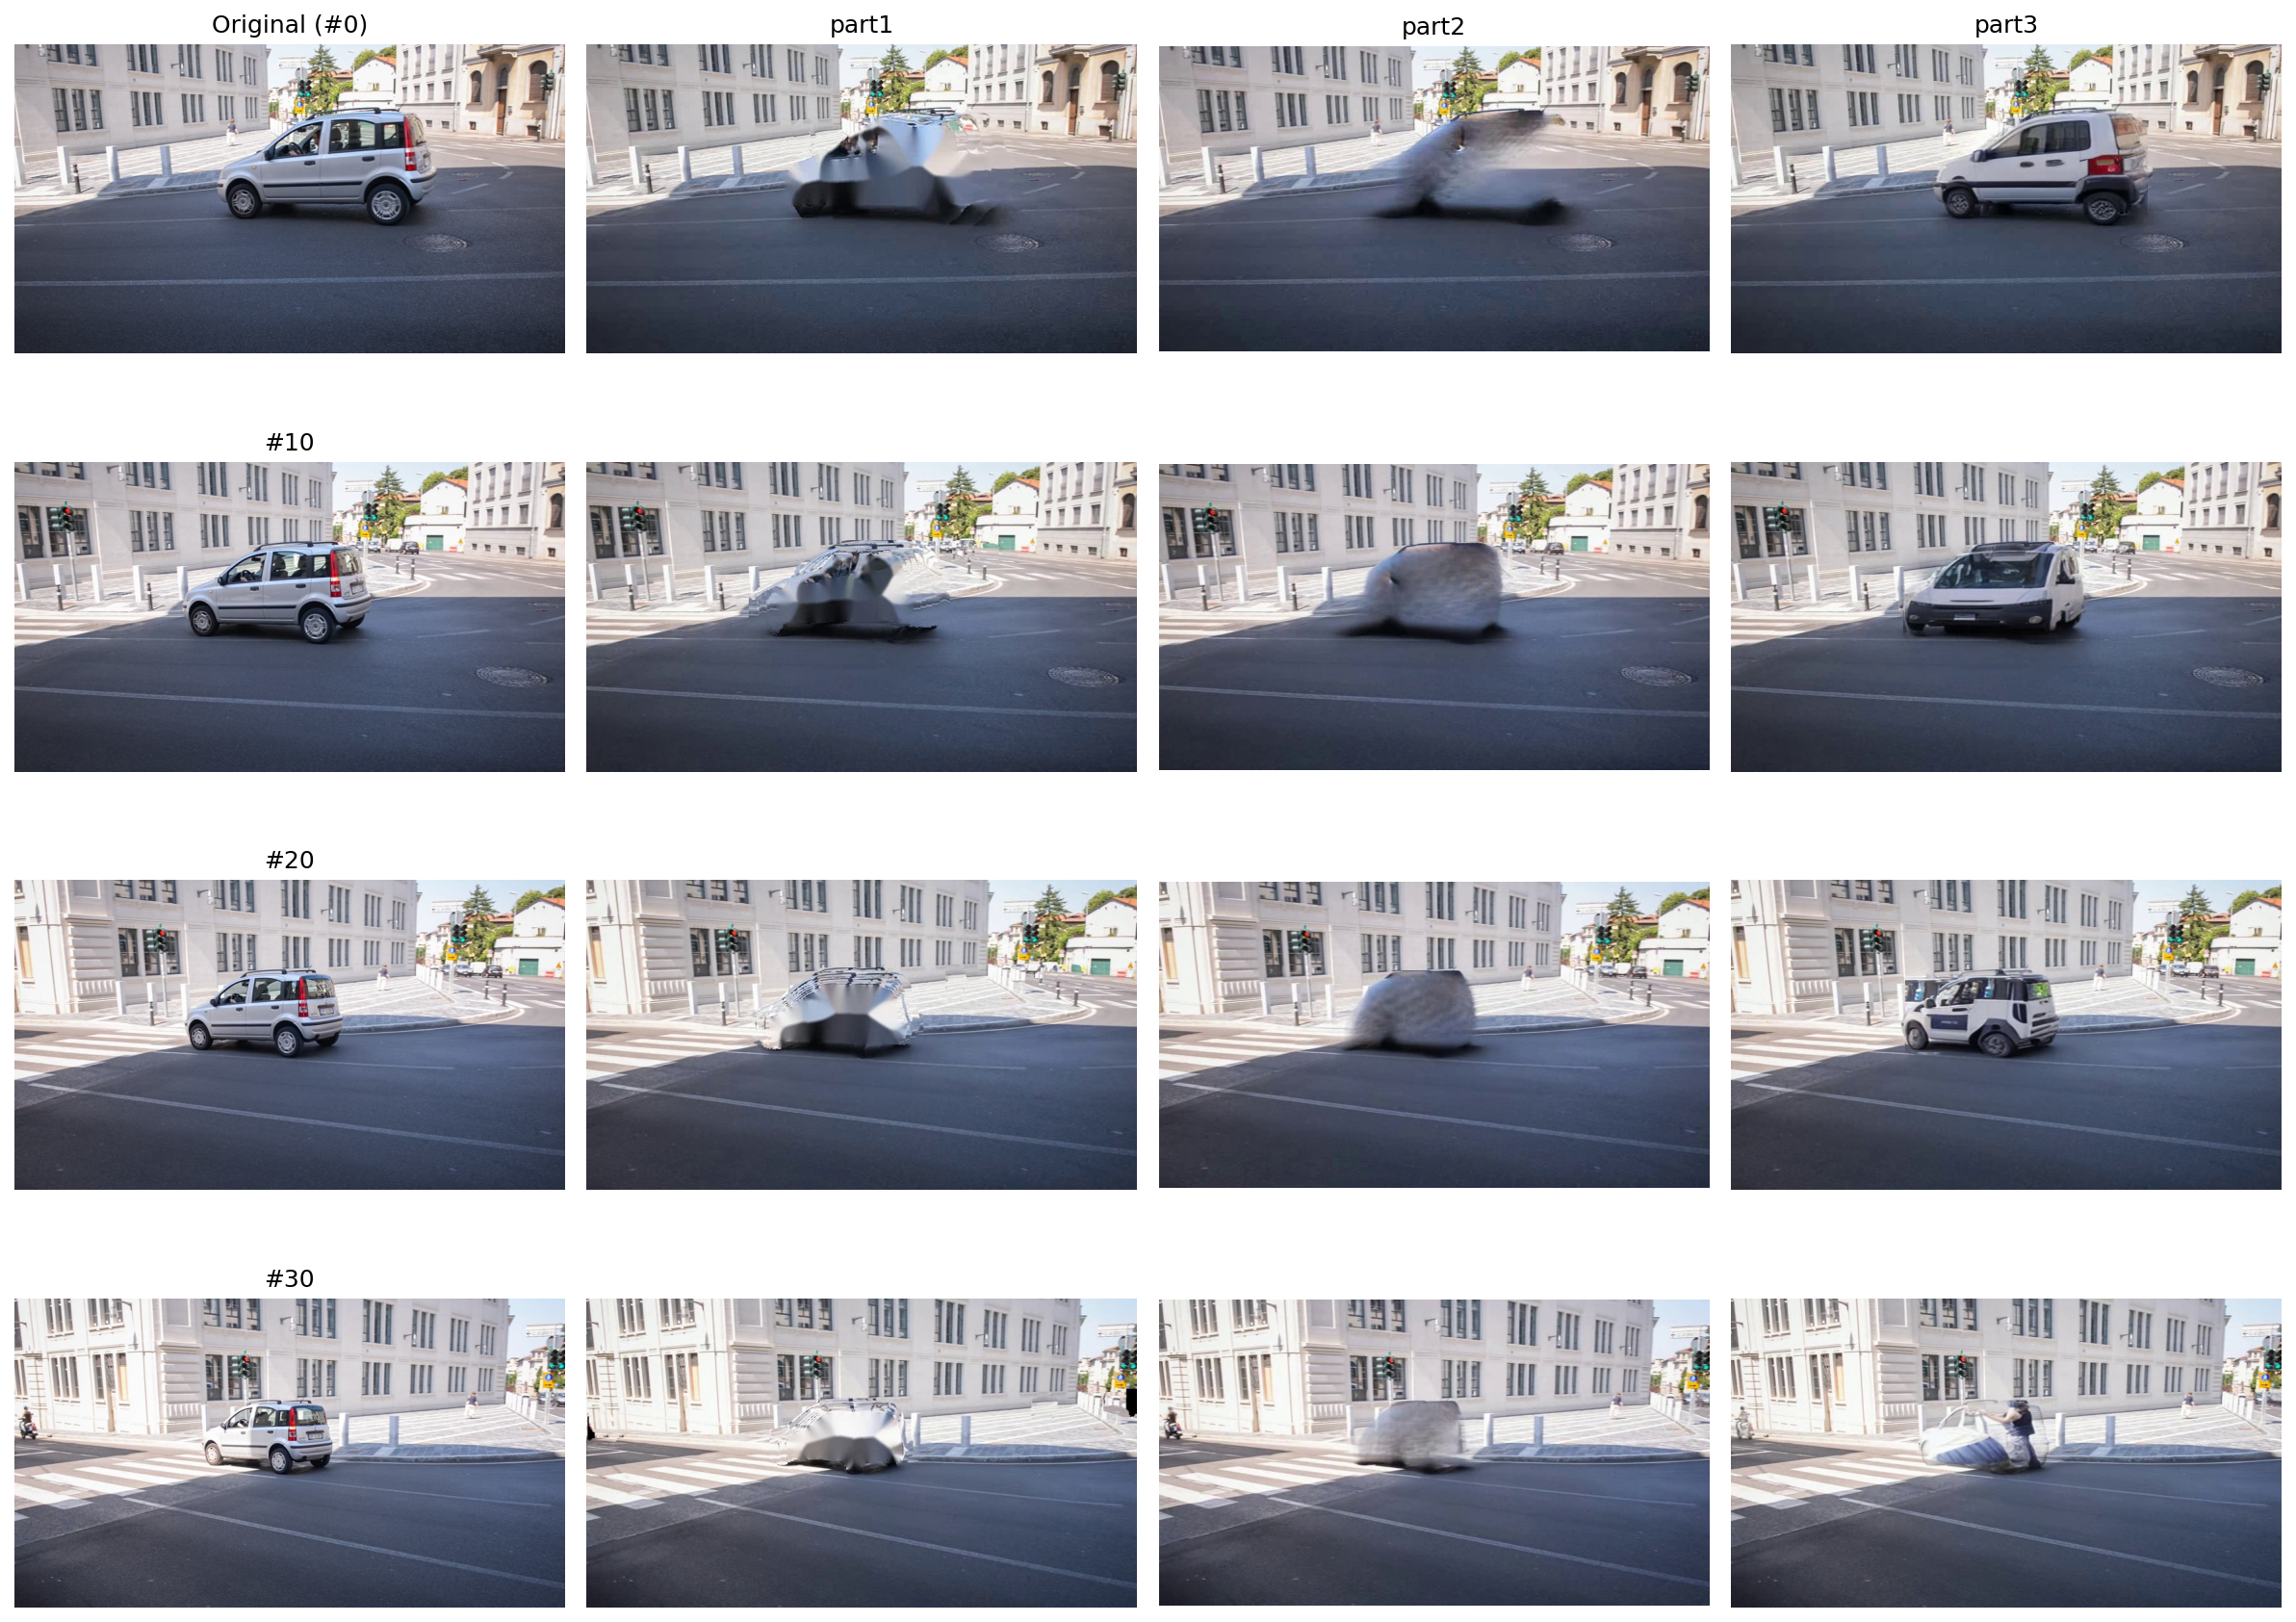
\includegraphics[width=\linewidth,height=0.16\textheight,keepaspectratio]{figures/comparison_car-shadow}
  \caption{Additional DAVIS result on \texttt{car-shadow}; cast shadows remain outside object masks.}
  \label{fig:qual_carshadow}
\end{figure}

\subsection{Failure cases and limitations}
Several limitations remain. First, shadows are generally not removed. This is expected because SAM~2 and DAVIS-style annotations segment object bodies, not cast shadows; ProPainter only repairs pixels inside the supplied mask. Adding shadow-aware mask expansion or a shadow detection model is future work. Second, diffusion inpainting can hallucinate plausible but temporally inconsistent texture. Keyframe propagation reduces flicker compared with per-frame generation, but it is not equivalent to a video diffusion model. Third, Part~1 still struggles with complex occlusions and fine background texture. Fourth, the RTX 4060 8GB GPU constrains resolution and batch size, forcing the wild clip to be resized. Finally, wild-video metrics are limited because no clean background or mask ground truth is available.

\subsection{Discussion}
The numbers in Tables~\ref{tab:mask}--\ref{tab:full} suggest a consistent trend. Part~2 is usually the best choice when the objective is temporally stable restoration with accurate masks, because SAM~2 and ProPainter are specialized for the same video setting. Part~3 is more useful when the missing region is large or unseen, because diffusion can synthesize plausible texture even when propagation alone fails. However, Part~3 must be treated carefully: a better masked PSNR does not always mean better perceived quality, since the synthesized texture may drift in identity or style across frames. On \texttt{dance-jump} and \texttt{tennis}, where motion is quick and foreground boundaries are thin, the strongest gain comes from the better mask tracking in Part~2 rather than from diffusion. On \texttt{bmx-trees} and \texttt{bus}, where background structure is more repetitive, Part~3’s generative branch performs better because it can reconstruct larger occluded patches with less visible patching.

These observations match the project spec. The final system is not a single universal solution; instead it is a progression of three methods with different trade-offs. Part~1 is simple and transparent, Part~2 is the most reliable for the mandatory data, and Part~3 provides a useful exploration of where generative models help and where they still fail.

\section{Conclusion}
\label{sec:conclusion}
We completed a progressive video object removal system with all three mandatory parts. The hand-crafted baseline demonstrates the limits of per-frame spatial inpainting and the benefit of temporal background propagation. The SAM~2 + ProPainter pipeline gives the most reliable perceptual video results and is our strongest practical method. The exploration branch shows that generative keyframe inpainting and seam-aware blending can improve masked PSNR, but also reveals current weaknesses of diffusion-based video restoration. Future work includes explicit shadow removal, real SAM~3 integration when tooling becomes available, geometry-aware dynamic masks from 4D foundation models, and video-native diffusion or joint mask-inpainting training for better temporal coherence.

{\small
\bibliographystyle{ieeetr}
\bibliography{references}
}

\end{document}
